\documentclass[11pt,a4paper]{article}

% Packages
\usepackage[utf8]{inputenc}
\usepackage[T1]{fontenc}
\usepackage{lmodern}
\usepackage[margin=2.5cm]{geometry}
\usepackage{graphicx}
\usepackage{booktabs}
\usepackage{longtable}
\usepackage{amsmath}
\usepackage{float}
\usepackage{caption}
\usepackage{subcaption}
\usepackage{xcolor}
\usepackage{listings}
\usepackage{fancyhdr}
\usepackage[hidelinks]{hyperref}
\usepackage{bookmark}

\graphicspath{{figures/}}
\hypersetup{pdftitle={EODP Unitary Test Reports}, pdfauthor={\studentname}}
\lstset{basicstyle=\ttfamily\small, breaklines=true, frame=single}

% Student data
\newcommand{\studentname}{V\'ictor Salas G\'omez}
\newcommand{\githuburl}{\url{https://github.com/SalasGomez/EODP}}

% Header and footer
\pagestyle{fancy}
\fancyhf{}
\lhead{EODP Unitary Test Reports}
\rhead{\studentname}
\cfoot{\thepage}

\title{\textbf{EODP Unitary Test Reports}\\[0.5em]
\large Earth Observation Data Processing\\Master in Space Engineering, UC3M}
\author{\studentname}
\date{\today}

\begin{document}

\maketitle
\thispagestyle{empty}

\tableofcontents
\listoffigures
\listoftables
\clearpage

\section{Introduction}
\label{sec:intro}

\subsection{Purpose}
This document reports the unitary tests of the EODP simulator.
The simulator models a passive optical multi-band imager with four VNIR bands.
It has three modules.
The Instrument Module (ISM) converts the input scene into digital numbers.
The Level-1B module (L1B) converts the digital numbers back into radiances.
The Level-1C module (L1C) projects the L1B radiances onto the MGRS grid.

Each test has its own section with the objective, the inputs, the execution, the results, the answer to the theoretical question and the conclusion.
The algorithms follow the ATBD \cite{atbd}.
The deliverables follow the guide to the subject \cite{guide}.

\subsection{Tests}
Table~\ref{tab:tests} lists the tests.

\begin{table}[H]
\centering
\caption{List of tests.}
\label{tab:tests}
\begin{tabular}{lll}
\toprule
Test & Module & Section \\
\midrule
EODP-TS-ISM & Instrument Module & \ref{sec:ism} \\
EODP-TS-L1B & Level-1B processing & \ref{sec:l1b} \\
EODP-TS-L1C & Level-1C processing & \ref{sec:l1c} \\
EODP-TS-E2E & End-to-end chain ISM, L1B and L1C & \ref{sec:e2e} \\
\bottomrule
\end{tabular}
\end{table}

\subsection{Pass criterion}
The outputs of the ISM, L1B and L1C tests are compared with the reference outputs of the teacher.
A test passes when the maximum relative difference of every output is lower than $10^{-3}\,\%$ \cite{guide}.
The relative difference of each file is
\begin{equation}
\varepsilon = \max_{i,j} \frac{\left| x_{ij} - x^{\mathrm{ref}}_{ij} \right|}{\left| x^{\mathrm{ref}}_{ij} \right|} \cdot 100 \, [\%].
\end{equation}
Pixels where the reference is zero are compared with the absolute difference.
The E2E test has no reference output. It is checked with the radiometric consistency of the chain.

\subsection{Test environment}
Table~\ref{tab:environment} shows the environment used to produce the results.
The source code is available in GitHub \cite{repo}.

\begin{table}[H]
\centering
\caption{Test environment.}
\label{tab:environment}
\begin{tabular}{ll}
\toprule
Item & Version \\
\midrule
Operating system & \texttt{Windows-10-10.0.26200-SP0} \\
Python & \texttt{3.11.9} \\
NumPy & \texttt{2.4.6} \\
SciPy & \texttt{1.17.1} \\
Matplotlib & \texttt{3.11.2} \\
netCDF4 & \texttt{1.7.5.1.post1} \\
mgrs & \texttt{1.5.0} \\
pyproj & \texttt{3.7.2} \\
Git commit & \texttt{39626a8} \\
\bottomrule
\end{tabular}

\end{table}

\subsection{References}
\begin{itemize}
\item \cite{atbd} EODP Algorithm Theoretical Baseline Document, revision 1.4.
\item \cite{guide} Guide to the Subject, revision 3.0.
\end{itemize}

\section{Test harness}
\label{sec:harness}

\subsection{Structure}
The harness has one folder per test inside \texttt{harness/}.
Each folder contains the four items required by the guide \cite{guide}.

\begin{itemize}
\item \texttt{test\_*.py}. The script that launches the test and generates the figures and tables.
\item \texttt{log/}. The log of the test script and the logs of the EODP modules of the final execution.
\item \texttt{output/}. All the outputs generated in the execution.
\item \texttt{figures/}. All the figures of the test. They are the same figures included in this report.
\end{itemize}

The folder \texttt{harness/common/} has the shared functions.
They handle the paths, the logs, the figures and the cross-validation.
The cross-validation tables of this report are written by the scripts. They are not typed by hand.

\begin{lstlisting}
harness/
  common/            harness_utils.py, environment.py
  EODP-TS-ISM/       test_ism.py, log/, output/, figures/
  EODP-TS-L1B/       test_l1b.py, log/, output/, figures/
  EODP-TS-L1C/       test_l1c.py, log/, output/, figures/
  EODP-TS-E2E/       test_e2e.py, log/, output/, figures/
\end{lstlisting}

\subsection{Execution}
The scripts run from the root of the repository with the Python environment of Table~\ref{tab:environment}.
The input data of the teacher is placed in \texttt{EODP\_TER\_2021/} and \texttt{EODP-TS-E2E/}.

\begin{lstlisting}
python harness/EODP-TS-ISM/test_ism.py
python harness/EODP-TS-L1B/test_l1b.py
python harness/EODP-TS-L1C/test_l1c.py
python harness/EODP-TS-E2E/test_e2e.py
\end{lstlisting}

The own outputs are written in the harness folders.
The reference outputs are never overwritten.

\subsection{Changes to the provided code}
The skeleton of the simulator was completed with the algorithms of the ATBD \cite{atbd}.
Some changes were needed to run it in the test environment.

\begin{itemize}
\item The main scripts use paths relative to the repository.
\item The log file path uses forward slashes. The logging configuration evaluates the path as a string and the Windows backslashes broke it.
\item The configuration files are loaded with a small loader. If the variable \texttt{EODP\_CONFIG\_DIR} is set, the configuration is read from that folder. The E2E test uses it to load the E2E configuration.
\item The unused \texttt{interp2d} imports were removed. The function no longer exists in recent SciPy versions.
\item The \texttt{mgrs} library is fixed to version 1.5.0. Later versions return the centre of the MGRS tile instead of its south-west corner. The reference outputs use the corner.
\item All the figures use the \texttt{classic} Matplotlib style and \LaTeX{} fonts.
\end{itemize}

\section{EODP-TS-ISM. Instrument Module}
\label{sec:ism}

\subsection{Objective}
The test validates the Instrument Module.
The ISM converts the input TOA spectral radiances into digital numbers in three stages \cite{atbd}.
\begin{itemize}
\item Optical stage. Spectral integration with the ISRF, conversion to irradiance and application of the system MTF.
\item Detection stage. Conversion to photons and electrons, PRNU, dark signal and bad or dead pixels.
\item Video chain. Conversion to volts and digitisation.
\end{itemize}
The test also answers two questions. Which MTF defines the system, and do the unit conversion factors reproduce the saved outputs.

\subsection{Inputs and configuration}
The input is the scene \texttt{gradient\_alt100\_act150/sgm\_toa.nc}.
It has 100 lines ALT, 150 columns ACT and 600 wavelengths from 400 to 999~nm.
The radiance grows linearly in the ACT direction.
Table~\ref{tab:ism_config} lists the main parameters of the default configuration.

\begin{table}[H]
\centering
\caption{Main ISM configuration parameters.}
\label{tab:ism_config}
\begin{tabular}{llr}
\toprule
Parameter & Symbol & Value \\
\midrule
Pixel size & $w$ & 30~\textmu m \\
Integration time & $t_{int}$ & 6.72~ms \\
Pupil diameter & $D$ & 0.150~m \\
Focal length & $f$ & 0.5262~m \\
Optical transmittance & $T_r$ & 0.99 \\
Central wavelengths & $\lambda$ & 490, 665, 865, 945~nm \\
Quantum efficiency & $QE$ & 0.8~e$^-$/ph \\
Full well capacity & $FWC$ & 420000~e$^-$ \\
Output conversion factor & $OCF$ & $5.4\times10^{-6}$~V/e$^-$ \\
ADC gain & $G$ & 0.56 \\
Bit depth & $N_{bits}$ & 12 \\
Voltage range & $V_{max}-V_{min}$ & 0.86~V \\
PRNU and DSNU factors & $k_{PRNU}$, $k_{DSNU}$ & 0.04, 0.2 \\
Bad and dead pixels & & 1.0~\%, 0.5~\% \\
\bottomrule
\end{tabular}
\end{table}

\subsection{Execution}
The script \texttt{harness/EODP-TS-ISM/test\_ism.py} runs the ISM with all the effects enabled.
It saves every intermediate output and the seven MTFs of each band.
Then it compares them with the reference outputs and generates the figures and tables of this section.

\subsection{Results}

\subsubsection{Cross-validation}
Tables~\ref{tab:ism_crossval_toa} and~\ref{tab:ism_crossval_mtf} show the maximum relative difference of every output with respect to the reference.
All the files are identical to the reference.
This includes the PRNU and the dark signal, which use random numbers with a fixed seed.

\begin{longtable}{lccccc}
\caption{ISM cross-validation of the TOA outputs. Maximum relative difference [\%] per band.}\label{tab:ism_crossval_toa}\\
\toprule
File & VNIR-0 & VNIR-1 & VNIR-2 & VNIR-3 & Result \\
\midrule
\endfirsthead
\toprule
File & VNIR-0 & VNIR-1 & VNIR-2 & VNIR-3 & Result \\
\midrule
\endhead
\texttt{ism\_toa\_isrf\_} & $0$ & $0$ & $0$ & $0$ & Pass \\
\texttt{ism\_toa\_optical\_} & $0$ & $0$ & $0$ & $0$ & Pass \\
\texttt{ism\_toa\_e\_} & $0$ & $0$ & $0$ & $0$ & Pass \\
\texttt{ism\_toa\_prnu\_} & $0$ & $0$ & $0$ & $0$ & Pass \\
\texttt{ism\_toa\_ds\_} & $0$ & $0$ & $0$ & $0$ & Pass \\
\texttt{ism\_toa\_detection\_} & $0$ & $0$ & $0$ & $0$ & Pass \\
\texttt{ism\_toa\_} & $0$ & $0$ & $0$ & $0$ & Pass \\
\bottomrule
\end{longtable}

\begin{longtable}{lccccc}
\caption{ISM cross-validation of the MTFs. Maximum relative difference [\%] per band.}\label{tab:ism_crossval_mtf}\\
\toprule
File & VNIR-0 & VNIR-1 & VNIR-2 & VNIR-3 & Result \\
\midrule
\endfirsthead
\toprule
File & VNIR-0 & VNIR-1 & VNIR-2 & VNIR-3 & Result \\
\midrule
\endhead
\texttt{Hdiff\_} & $0$ & $0$ & $0$ & $0$ & Pass \\
\texttt{Hdefoc\_} & $0$ & $0$ & $0$ & $0$ & Pass \\
\texttt{Hwfe\_} & $0$ & $0$ & $0$ & $0$ & Pass \\
\texttt{Hdet\_} & $0$ & $0$ & $0$ & $0$ & Pass \\
\texttt{Hsmear\_} & $0$ & $0$ & $0$ & $0$ & Pass \\
\texttt{Hmotion\_} & $0$ & $0$ & $0$ & $0$ & Pass \\
\texttt{Hsys\_} & $0$ & $0$ & $0$ & $0$ & Pass \\
\bottomrule
\end{longtable}


\subsubsection{Signal through the stages}
Figure~\ref{fig:ism_stages} shows the central ALT line after each stage.
The radiance after the ISRF is a straight line, as the input scene.
The MTF modifies the first and last columns. The FFT treats the image as periodic, so the bright last column is mixed with the dark first one.
The detection stage adds the stripes of the PRNU and the DSNU.
In VNIR-2 and VNIR-3 the signal reaches the full well capacity of 420000~e$^-$.
After the video chain VNIR-1, VNIR-2 and VNIR-3 saturate at 4095~DN.

\begin{figure}[H]
\centering
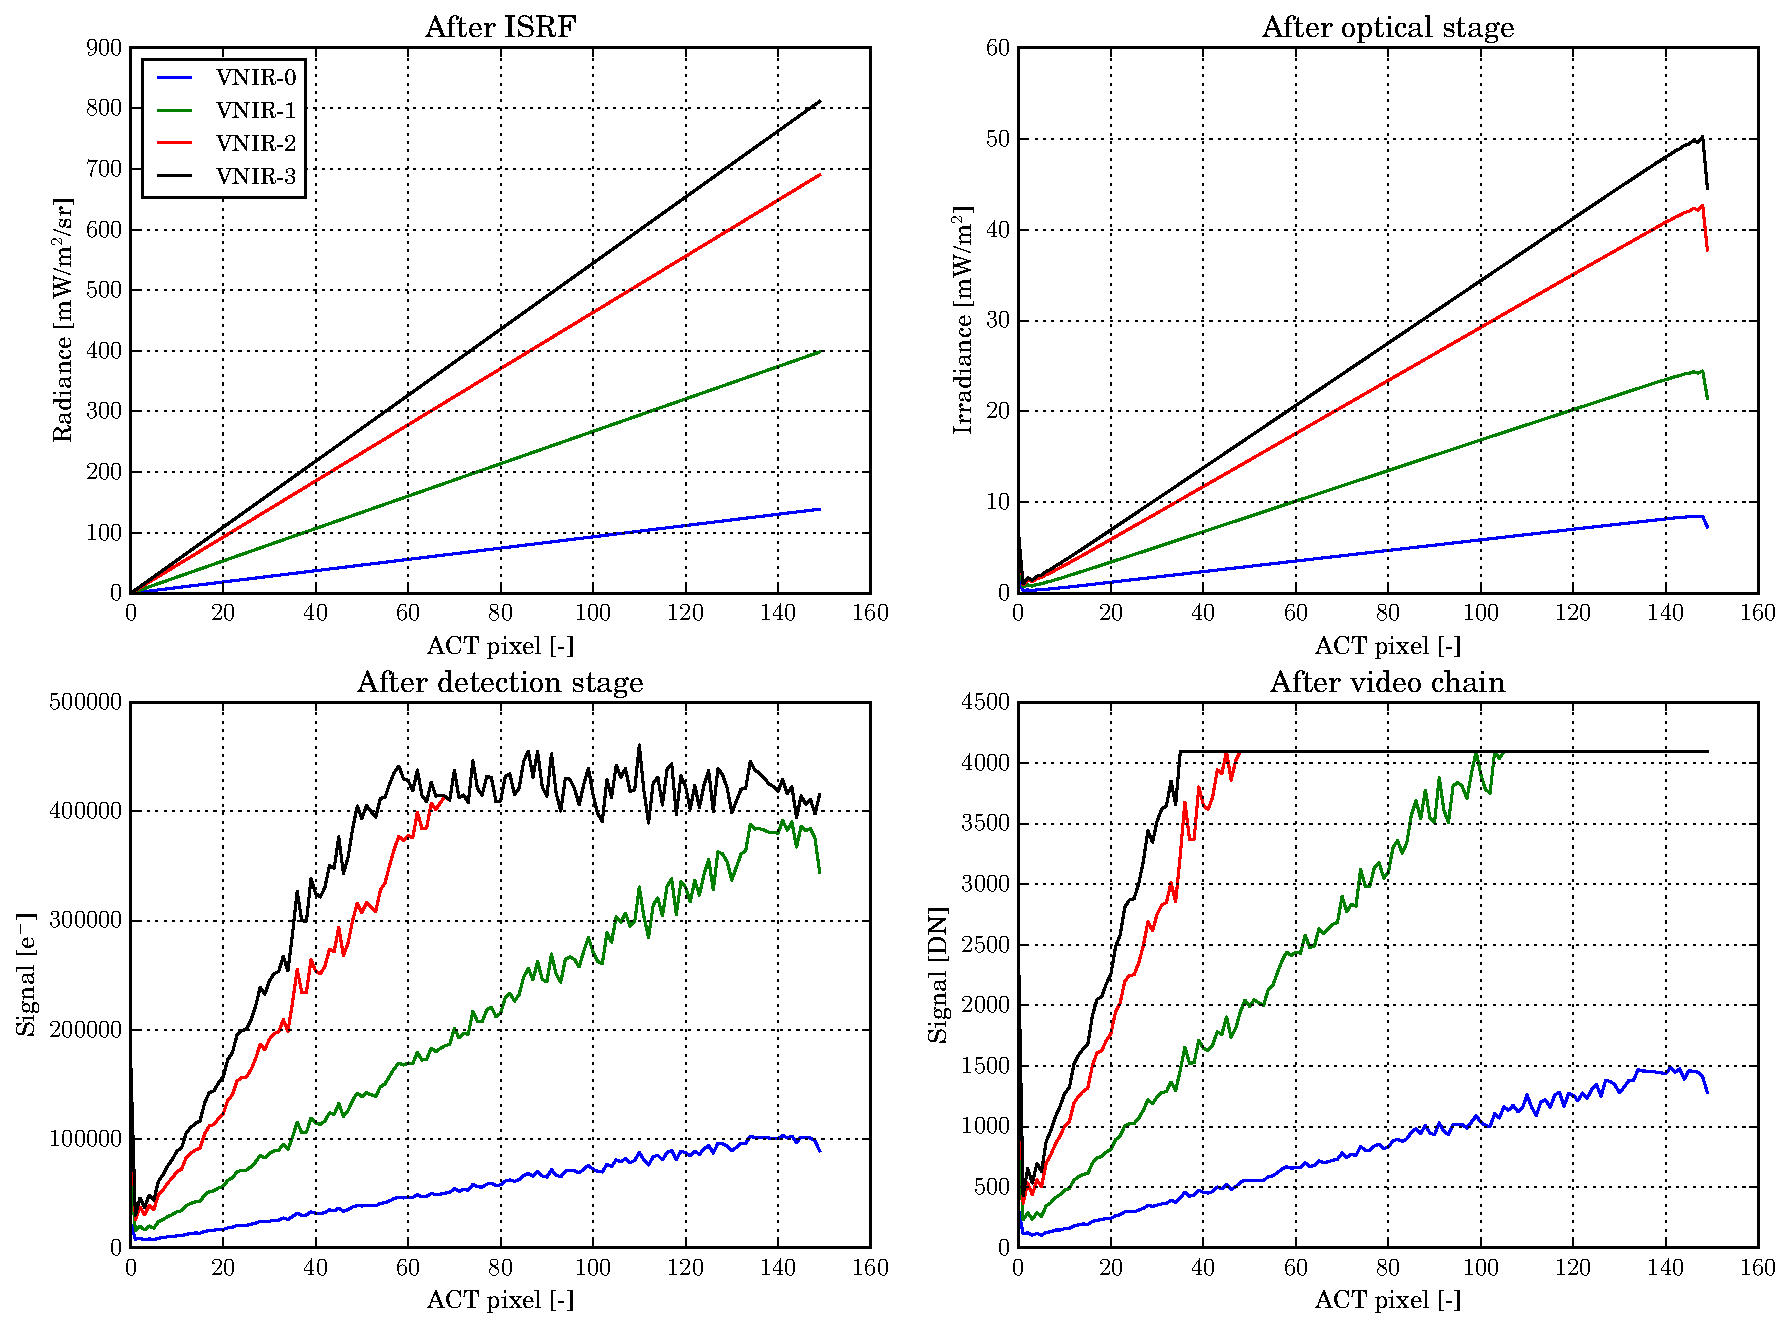
\includegraphics[width=\textwidth]{ism_stages}
\caption{ISM. Central ALT line after each stage for the four bands.}
\label{fig:ism_stages}
\end{figure}

\subsubsection{MTF}
Figures~\ref{fig:ism_mtf_0} to~\ref{fig:ism_mtf_3} show the cuts of the MTF in the ACT and ALT directions up to the Nyquist frequency.
The frequencies are normalised with the inverse of the pixel width, so Nyquist is at 0.5.
Table~\ref{tab:ism_mtf_nyquist} gives the value of each contributor at the last sample before Nyquist.

\begin{figure}[H]
\centering
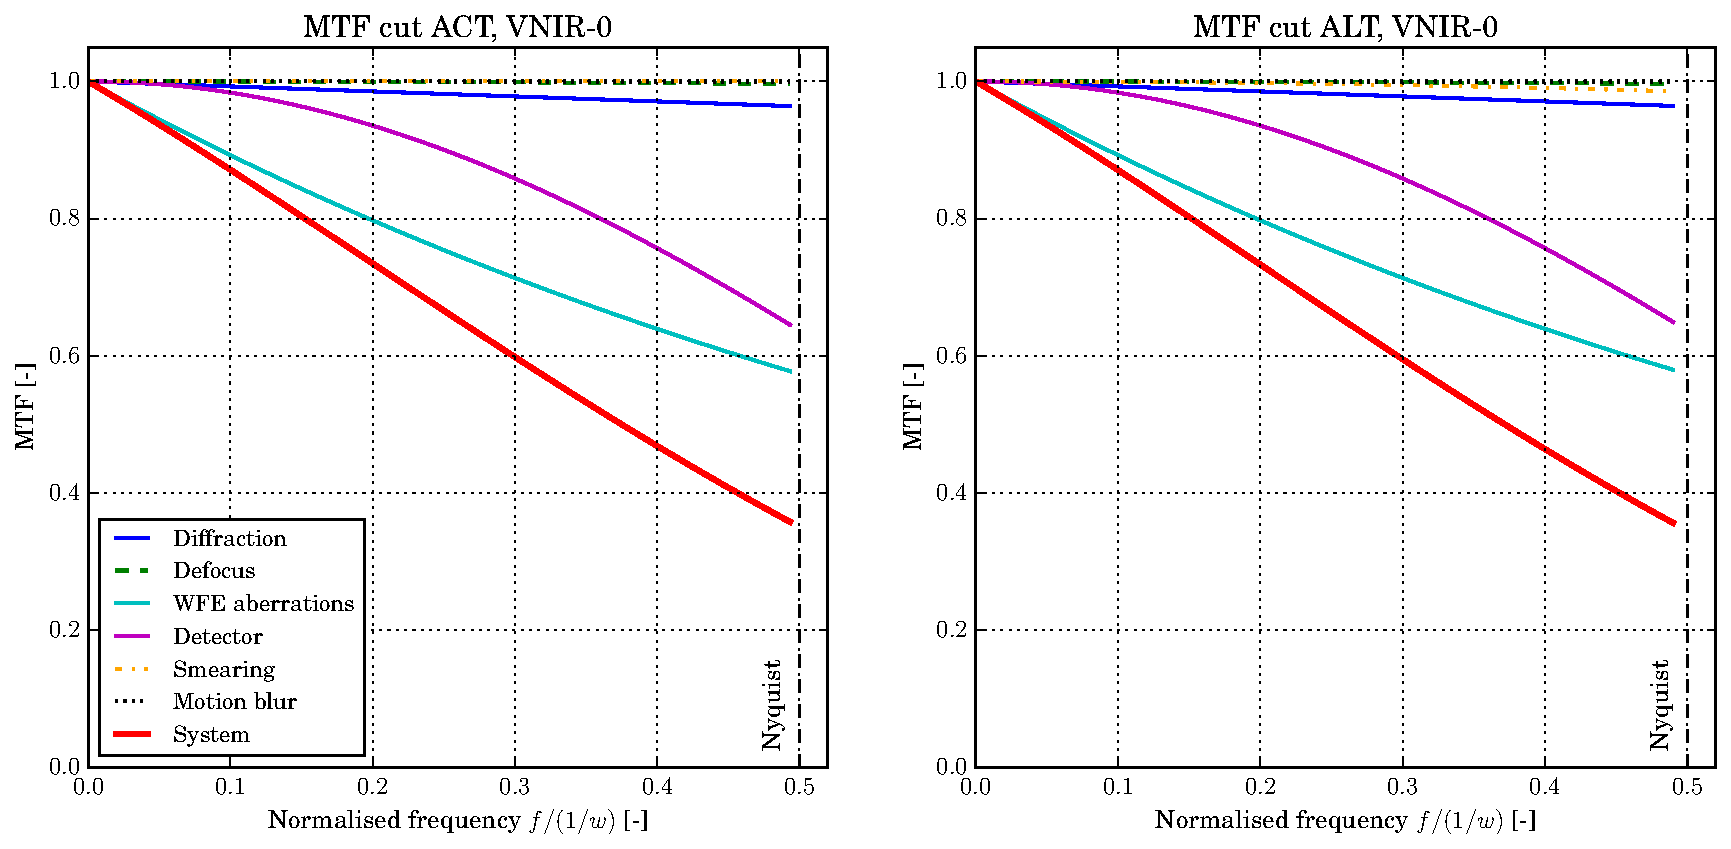
\includegraphics[width=\textwidth]{ism_mtf_VNIR-0}
\caption{ISM. MTF cuts ACT and ALT, VNIR-0.}
\label{fig:ism_mtf_0}
\end{figure}

\begin{figure}[H]
\centering
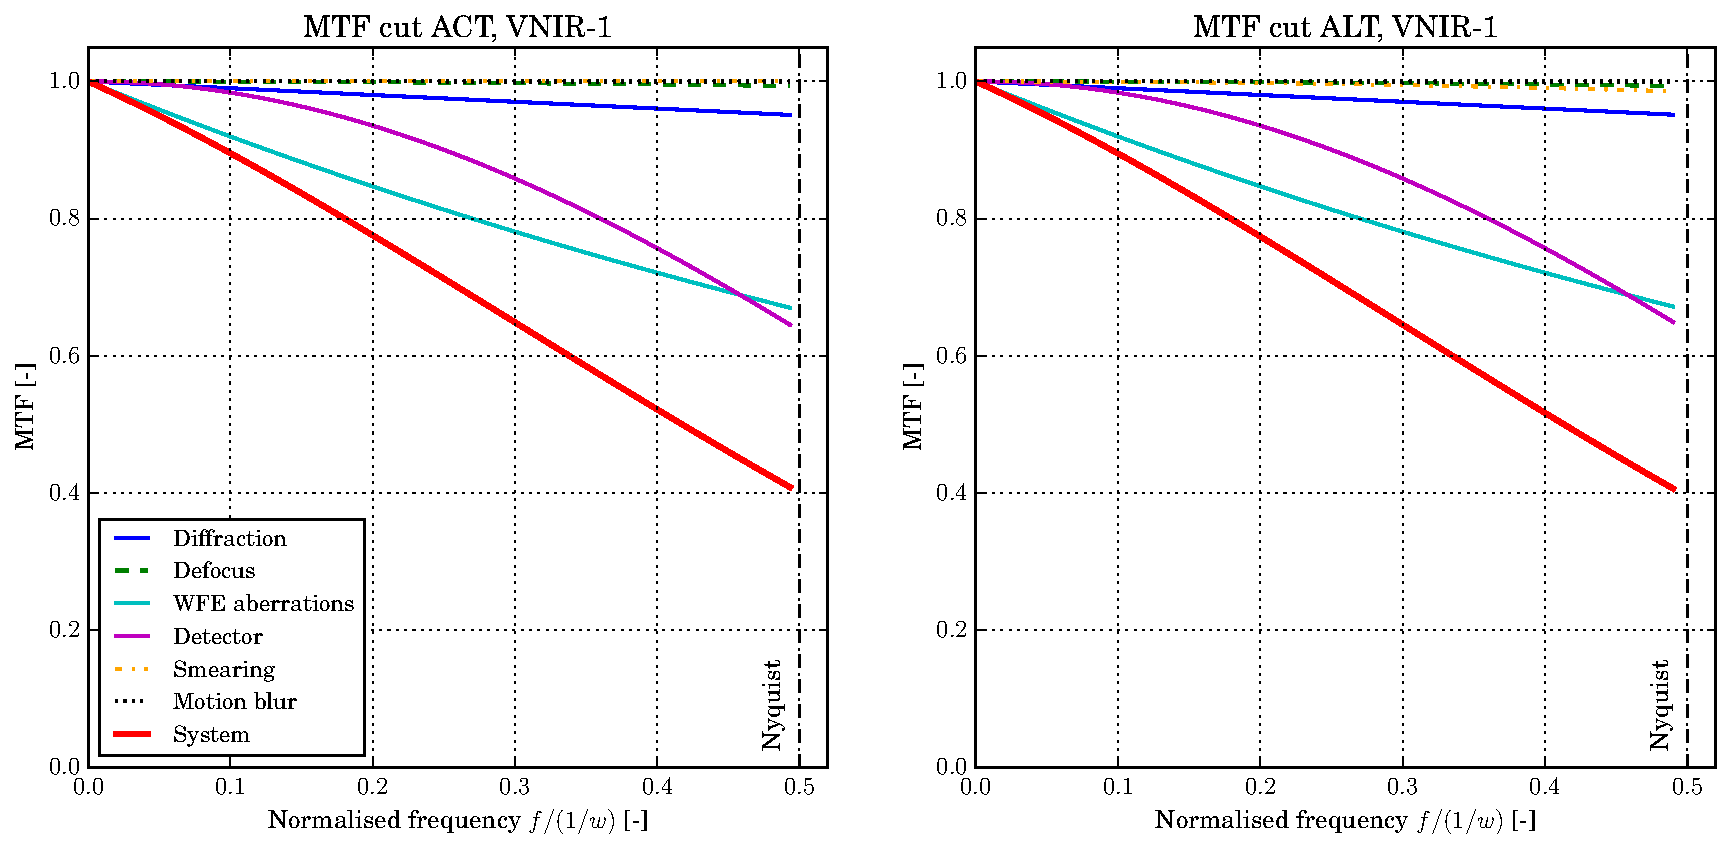
\includegraphics[width=\textwidth]{ism_mtf_VNIR-1}
\caption{ISM. MTF cuts ACT and ALT, VNIR-1.}
\label{fig:ism_mtf_1}
\end{figure}

\begin{figure}[H]
\centering
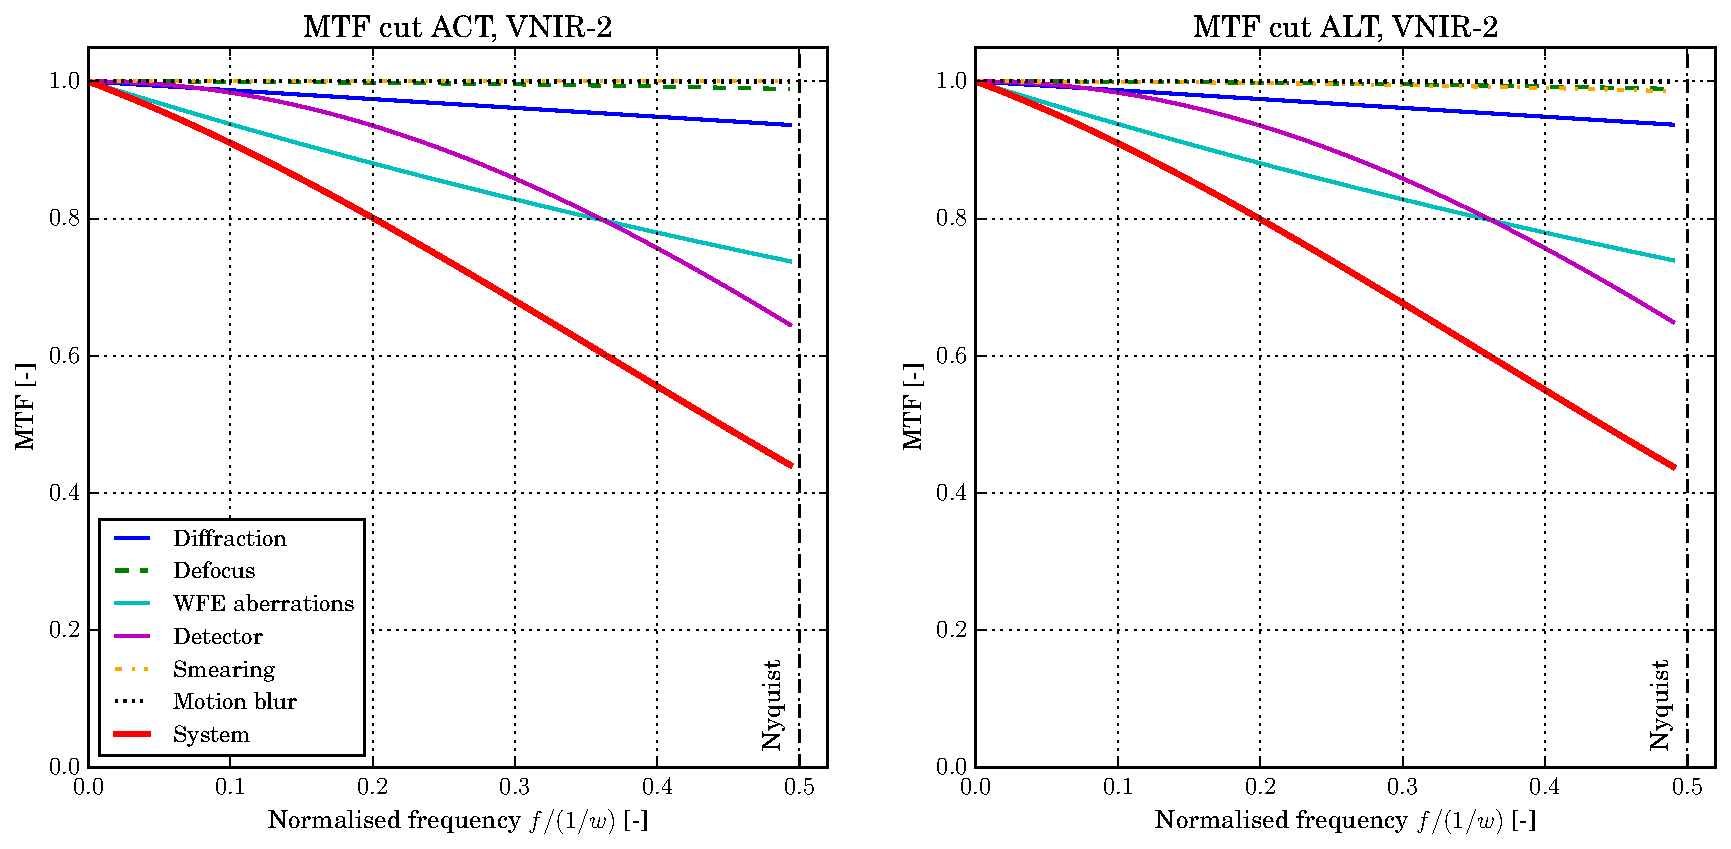
\includegraphics[width=\textwidth]{ism_mtf_VNIR-2}
\caption{ISM. MTF cuts ACT and ALT, VNIR-2.}
\label{fig:ism_mtf_2}
\end{figure}

\begin{figure}[H]
\centering
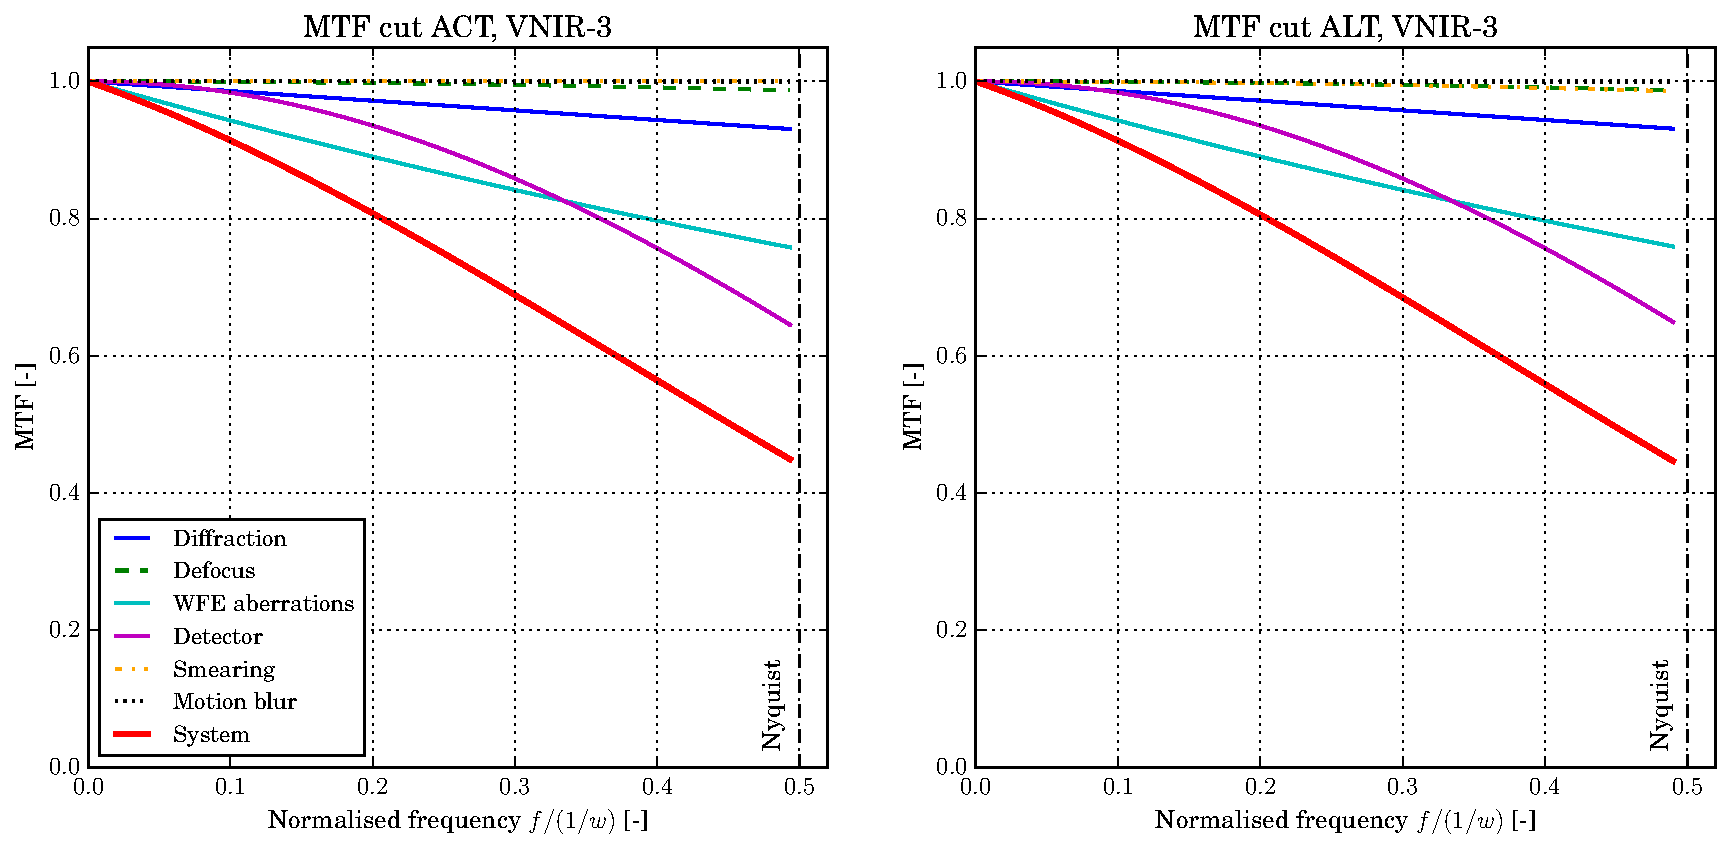
\includegraphics[width=\textwidth]{ism_mtf_VNIR-3}
\caption{ISM. MTF cuts ACT and ALT, VNIR-3.}
\label{fig:ism_mtf_3}
\end{figure}

\begin{table}[H]
\centering
\small
\caption{MTF of each contributor at the last sample before Nyquist.}
\label{tab:ism_mtf_nyquist}
\begin{tabular}{lcccccccc}
\toprule
 & \multicolumn{2}{c}{VNIR-0} & \multicolumn{2}{c}{VNIR-1} & \multicolumn{2}{c}{VNIR-2} & \multicolumn{2}{c}{VNIR-3} \\
MTF & ACT & ALT & ACT & ALT & ACT & ALT & ACT & ALT \\
\midrule
Diffraction & 0.964 & 0.964 & 0.951 & 0.951 & 0.936 & 0.937 & 0.931 & 0.931 \\
Defocus & 0.996 & 0.996 & 0.993 & 0.993 & 0.989 & 0.989 & 0.987 & 0.987 \\
WFE aberrations & 0.577 & 0.580 & 0.670 & 0.672 & 0.738 & 0.739 & 0.758 & 0.759 \\
Detector & 0.645 & 0.649 & 0.645 & 0.649 & 0.645 & 0.649 & 0.645 & 0.649 \\
Smearing & 1.000 & 0.986 & 1.000 & 0.986 & 1.000 & 0.986 & 1.000 & 0.986 \\
Motion blur & 1.000 & 1.000 & 1.000 & 1.000 & 1.000 & 1.000 & 1.000 & 1.000 \\
System & 0.358 & 0.356 & 0.408 & 0.406 & 0.441 & 0.438 & 0.449 & 0.447 \\
\bottomrule
\end{tabular}

\end{table}

\subsubsection{Unit conversion at the central pixel}
Each conversion of the ISM is a scalar factor for a given band.
Table~\ref{tab:ism_units_factors} lists the factors.
They are
\begin{align}
I &= L \cdot T_r \frac{\pi}{4}\left(\frac{D}{f}\right)^2, &
N_{ph} &= I \cdot \frac{A_{pix}\, t_{int}\, \lambda}{h c}, &
N_e &= N_{ph} \cdot QE, \\
V &= N_e \cdot OCF \cdot G, &
DN &= \mathrm{round}\left( V \cdot \frac{2^{N_{bits}}-1}{V_{max}-V_{min}} \right). & &
\end{align}
The irradiance is converted from mW to W before the conversion to photons.
The factors are applied to the radiance of the central pixel [50, 75] of \texttt{ism\_toa\_isrf}.
The result is compared with the two outputs that the code saves in these units. They are the electrons of \texttt{ism\_toa\_e} and the digital numbers of \texttt{ism\_toa}.
Irradiance, photons and volts are not saved.
Table~\ref{tab:ism_units_check} shows the comparison.

\begin{table}[H]
\centering
\small
\caption{Unit conversion factors per band. The two largest factors of each band are in bold.}
\label{tab:ism_units_factors}
\begin{tabular}{llcccc}
\toprule
Step & Units & VNIR-0 & VNIR-1 & VNIR-2 & VNIR-3 \\
\midrule
Radiance $\rightarrow$ irradiance & [sr] & $6.32\times10^{-2}$ & $6.32\times10^{-2}$ & $6.32\times10^{-2}$ & $6.32\times10^{-2}$ \\
Irradiance $\rightarrow$ photons & [ph m$^2$/mW] & $\mathbf{1.49\times10^{4}}$ & $\mathbf{2.02\times10^{4}}$ & $\mathbf{2.63\times10^{4}}$ & $\mathbf{2.88\times10^{4}}$ \\
Photons $\rightarrow$ electrons & [e$^-$/ph] & $8.00\times10^{-1}$ & $8.00\times10^{-1}$ & $8.00\times10^{-1}$ & $8.00\times10^{-1}$ \\
Electrons $\rightarrow$ volts & [V/e$^-$] & $3.02\times10^{-6}$ & $3.02\times10^{-6}$ & $3.02\times10^{-6}$ & $3.02\times10^{-6}$ \\
Volts $\rightarrow$ DN & [DN/V] & $\mathbf{4.76\times10^{3}}$ & $\mathbf{4.76\times10^{3}}$ & $\mathbf{4.76\times10^{3}}$ & $\mathbf{4.76\times10^{3}}$ \\
\bottomrule
\end{tabular}

\end{table}

\begin{table}[H]
\centering
\small
\caption{Analytic conversion at the central pixel compared with the saved outputs.}
\label{tab:ism_units_check}
\begin{tabular}{lcccc}
\toprule
Quantity & VNIR-0 & VNIR-1 & VNIR-2 & VNIR-3 \\
\midrule
Radiance $L$ [mW/m$^2$/sr] & 69.8533 & 200.3996 & 347.5041 & 408.5177 \\
Electrons, analytic from $L$ [e$^-$] & 52676.1 & 205092.4 & 462601.4 & 594119.3 \\
Electrons, \texttt{ism\_toa\_e} [e$^-$] & 52673.4 & 205082.8 & 420000.0 & 420000.0 \\
Electrons, analytic from optical TOA [e$^-$] & 52673.4 & 205082.8 & 462581.2 & 594093.7 \\
DN, analytic from $L$ [DN] & 758 & 2953 & 6661 & 8555 \\
DN, \texttt{ism\_toa} [DN] & 804 & 2985 & 4095 & 4095 \\
DN, analytic from detection TOA, saturated [DN] & 804 & 2985 & 4095 & 4095 \\
\midrule
Rel. diff. electrons [\%] & -0.005 & -0.005 & -9.209 & -29.307 \\
Rel. diff. DN [\%] & 6.069 & 1.084 & -38.523 & -52.133 \\
\bottomrule
\end{tabular}

\end{table}

The analytic values do not match the saved outputs exactly.
Some steps of the ISM change the value of the signal but not its units.
\begin{itemize}
\item The MTF is applied between the irradiance and the photons. It explains the difference of $-0.005\,\%$ in the electrons of VNIR-0 and VNIR-1. If the chain starts from the optical TOA, which already includes the MTF, the electrons match \texttt{ism\_toa\_e}.
\item The FWC limits the electrons to 420000~e$^-$. In VNIR-2 and VNIR-3 the analytic value is higher, so the saved value is the FWC.
\item The PRNU, the dark signal and the bad pixels are applied after \texttt{ism\_toa\_e}. They change the DN by $+6\,\%$ in VNIR-0 and by $+1\,\%$ in VNIR-1. If the chain starts from the detection TOA, the DN match \texttt{ism\_toa}.
\item The digitisation rounds the signal and saturates it at $2^{12}-1 = 4095$~DN. VNIR-2 and VNIR-3 are saturated at the central pixel.
\end{itemize}

The two most significant steps are the ones with the largest factors.
They are the conversion from irradiance to photons, with a factor between $1.5\times10^{4}$ and $2.9\times10^{4}$, and the conversion from volts to DN, with a factor of $4.76\times10^{3}$.
The first factor grows with the wavelength because a photon of longer wavelength carries less energy.

\subsection{Theoretical question. Which MTF defines the system?}
The system MTF is the product of the six contributors.
The contributor with the lowest value at Nyquist drives the system MTF down the most.
Table~\ref{tab:ism_mtf_nyquist} shows two dominant terms.
\begin{itemize}
\item The detector MTF is $|\mathrm{sinc}(f_n)|$. It only depends on the pixel width. At Nyquist it is close to $2/\pi \approx 0.64$ in all the bands.
\item The wavefront error MTF depends on $(W/\lambda)^2$. It is lower at short wavelengths. In VNIR-0 it is 0.58 and it is the lowest contributor. In the other bands it is between 0.67 and 0.76.
\end{itemize}
So the detector defines the system MTF in VNIR-1, VNIR-2 and VNIR-3, and the wavefront error aberrations define it in VNIR-0.
The diffraction MTF stays above 0.93. The optics cut-off frequency $D/(\lambda f)$ is between 9 and 17 times the sampling frequency $1/w$. Nyquist is then at only 3 to 6~\% of the cut-off frequency.
Defocus, smearing and motion blur are close to one. Smearing only acts in the ALT direction.
The system MTF at Nyquist is between 0.36 and 0.45. This value is high, so the system is prone to aliasing.


\textbf{EODP-TS-ISM: PASS.}

\section{EODP-TS-L1B. Level-1B processing}
\label{sec:l1b}

\subsection{Objective}
The test validates the L1B module.
The L1B converts the digital numbers of the ISM back into TOA radiances in two steps \cite{atbd}.
\begin{itemize}
\item Equalization. It removes the offset and the gain of each pixel: $DN_{eq} = (DN - eq_{add}) / eq_{mult}$.
\item Restoration. It applies the absolute radiometric gain of the band: $L_{L1B} = DN_{eq} \cdot g$.
\end{itemize}

\subsection{Inputs and configuration}
The input is the ISM output in \texttt{EODP\_TER\_2021/EODP-TS-L1B/input}.
It contains \texttt{ism\_toa} in DN and \texttt{ism\_toa\_isrf}, the radiance before the instrument effects.
The equalization factors are the files \texttt{eq\_add} and \texttt{eq\_mult} of the auxiliary folder. They have one value per ACT pixel.
The absolute gains are 0.0921, 0.0679, 0.0522 and 0.0478 mW/m$^2$/sr/DN for the four bands.

\subsection{Execution}
The script \texttt{harness/EODP-TS-L1B/test\_l1b.py} runs the L1B twice.
The first run has \texttt{do\_equalization = False}. The second run has \texttt{do\_equalization = True}. The second run is the one cross-validated.

\subsection{Results}

\subsubsection{Cross-validation}
Table~\ref{tab:l1b_crossval} shows the comparison of the equalized DN and the L1B radiances with the reference.
All the files are identical to the reference.

\begin{longtable}{lccccc}
\caption{L1B cross-validation with equalization. Maximum relative difference [\%] per band.}\label{tab:l1b_crossval}\\
\toprule
File & VNIR-0 & VNIR-1 & VNIR-2 & VNIR-3 & Result \\
\midrule
\endfirsthead
\toprule
File & VNIR-0 & VNIR-1 & VNIR-2 & VNIR-3 & Result \\
\midrule
\endhead
\texttt{l1b\_toa\_eq\_} & $0$ & $0$ & $0$ & $0$ & Pass \\
\texttt{l1b\_toa\_} & $0$ & $0$ & $0$ & $0$ & Pass \\
\bottomrule
\end{longtable}


\subsubsection{Calibration plot}
Figure~\ref{fig:l1b_calibration} shows the central ALT line of three images.
The black line is the TOA after the ISRF. It is the radiance that enters the instrument and it is taken as the truth.
The red line is the L1B without equalization. The blue line is the L1B with equalization.

\begin{figure}[H]
\centering
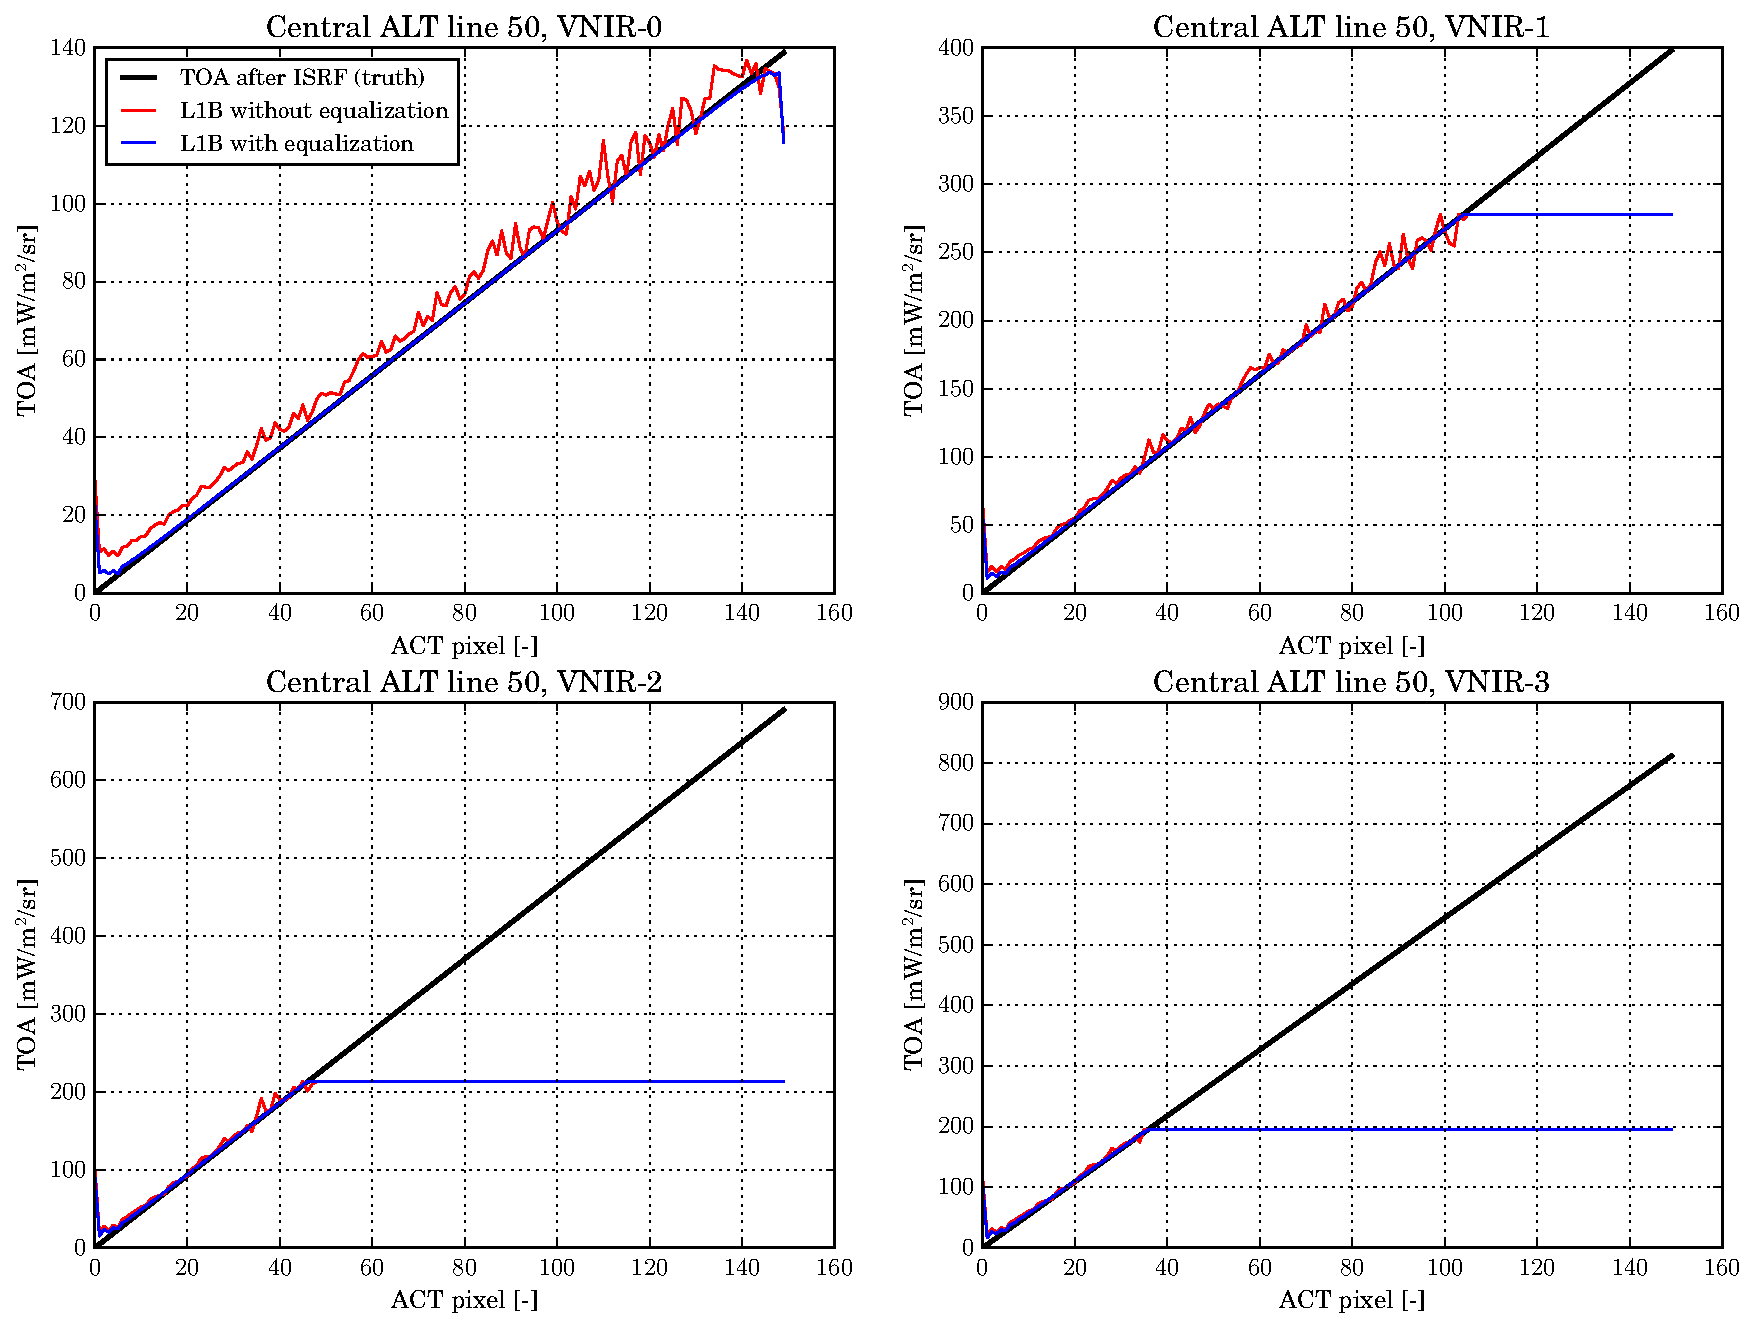
\includegraphics[width=\textwidth]{l1b_calibration}
\caption{L1B. TOA after the ISRF, L1B without equalization and L1B with equalization. Central ALT line.}
\label{fig:l1b_calibration}
\end{figure}

Without equalization the L1B shows the stripes of the PRNU and the DSNU. It is also shifted above the truth because the dark signal adds a positive offset. The shift is clear in VNIR-0, where the signal is low.
With equalization the stripes and the offset disappear and the L1B follows the truth.
Two differences remain.
The first and last columns differ because of the MTF edge effect of the ISM.
In VNIR-1, VNIR-2 and VNIR-3 the L1B becomes flat from a certain column. The L1B is ``blocked'' at a constant value.
This happens because the ISM saturated these pixels at the FWC and at 4095~DN (Section~\ref{sec:ism}). The information above saturation is lost and the L1B cannot recover it.
The flat level is the radiance that corresponds to 4095~DN after the equalization and the gain.

Table~\ref{tab:l1b_errors} gives the median relative error with respect to the truth.
Saturated pixels and the two columns of each border are excluded.
The median is used because the first columns have a radiance close to zero, where any small difference gives a large relative error.
The equalization reduces the error in all the bands.

\begin{table}[H]
\centering
\caption{L1B median relative error with respect to the TOA after the ISRF, and fraction of saturated pixels.}
\label{tab:l1b_errors}
\begin{tabular}{lccc}
\toprule
Band & Error without eq. [\%] & Error with eq. [\%] & Saturated pixels [\%] \\
\midrule
VNIR-0 & 7.494 & 0.233 & 0.0 \\
VNIR-1 & 4.116 & 0.166 & 30.7 \\
VNIR-2 & 4.216 & 0.946 & 68.7 \\
VNIR-3 & 5.047 & 1.655 & 76.7 \\
\bottomrule
\end{tabular}

\end{table}

\subsection{Theoretical question. What is calibration?}
Calibration is the process that finds the parameters which relate the instrument output to the physical quantity observed.
The instrument does not measure radiance. It produces digital numbers. Each pixel has its own response, with an offset from the dark signal and a gain from the PRNU.
The calibration has two parts.
\begin{itemize}
\item Relative calibration. It finds the offset and the gain of each pixel, so that all the pixels give the same output for the same input. These are the equalization factors $eq_{add}$ and $eq_{mult}$. The offset is measured with dark images, without illumination. The gain is measured with a uniform scene.
\item Absolute calibration. It finds the gain $g$ that converts the equalized DN into radiance. It is measured with a source of known radiance, such as an integrating sphere on ground or the Sun with a diffuser in flight.
\end{itemize}
The calibration parameters are measured in the calibration campaigns and stored in a characterisation database.
The L1B processing does not compute them. It only applies them.
Figure~\ref{fig:l1b_calibration} shows the effect. Without the relative calibration the image has stripes and an offset. With it the L1B recovers the input radiance up to the saturation level.

\subsection{Conclusion}
The L1B outputs with equalization match the reference with a relative difference of zero.
The equalization removes the PRNU and DSNU stripes.
\textbf{EODP-TS-L1B: PASS.}

\section{EODP-TS-L1C. Level-1C processing}
\label{sec:l1c}

\subsection{Objective}
The test validates the L1C module.
The L1C projects the L1B radiances onto the MGRS grid \cite{atbd}. The steps are the following.
\begin{enumerate}
\item Build a 2D spline interpolant of the L1B radiance as a function of latitude and longitude (\texttt{bisplrep}).
\item Convert every L1B coordinate into an MGRS tile with a precision of 100~m and keep the unique tiles.
\item Convert each tile back to latitude and longitude. The \texttt{mgrs} library \cite{mgrs} returns the south-west corner of the tile.
\item Evaluate the interpolant at these coordinates (\texttt{bisplev}). The result is the L1C radiance.
\end{enumerate}

\subsection{Inputs and configuration}
The inputs are the geolocation of the GM in \texttt{input/gm\_alt100\_act\_150} and the L1B radiances in \texttt{input/l1b\_output}.
Both are matrices of 100 lines by 150 columns.
The MGRS precision is 3, which gives tiles of 100~m.

\subsection{Execution}
The script \texttt{harness/EODP-TS-L1C/test\_l1c.py} runs the L1C with both input folders separated by a comma.
The L1C output is a list of points. Its order changes in each run because the tiles are stored in a Python set.
For this reason each reference point is matched with the closest output point before the comparison.

\subsection{Results}

\subsubsection{Cross-validation}
Table~\ref{tab:l1c_crossval} shows the comparison.
The number of points is the same. Every reference point has an output point at zero distance, and the radiances are identical.

\begin{table}[H]
\centering
\small
\caption{L1C cross-validation after matching the points by coordinates.}
\label{tab:l1c_crossval}
\begin{tabular}{lccccc}
\toprule
Band & Points ref. & Points output & Max. distance [m] & Max. rel. diff. [\%] & Result \\
\midrule
VNIR-0 & 3129 & 3129 & $0$ & $0$ & Pass \\
VNIR-1 & 3129 & 3129 & $0$ & $0$ & Pass \\
VNIR-2 & 3129 & 3129 & $0$ & $0$ & Pass \\
VNIR-3 & 3129 & 3129 & $0$ & $0$ & Pass \\
\bottomrule
\end{tabular}

\end{table}

\subsubsection{L1B and L1C grids}
Figure~\ref{fig:l1c_grids} shows both grids in the same plot.
The L1B grid follows the geometry of the sensor. It is tilted with respect to the meridians because of the orbit inclination.
The L1C grid is regular in UTM coordinates. Its points are aligned with the north and the east.
The L1C grid is coarser. There are 3129 L1C points against 15000 L1B points.

\begin{figure}[H]
\centering
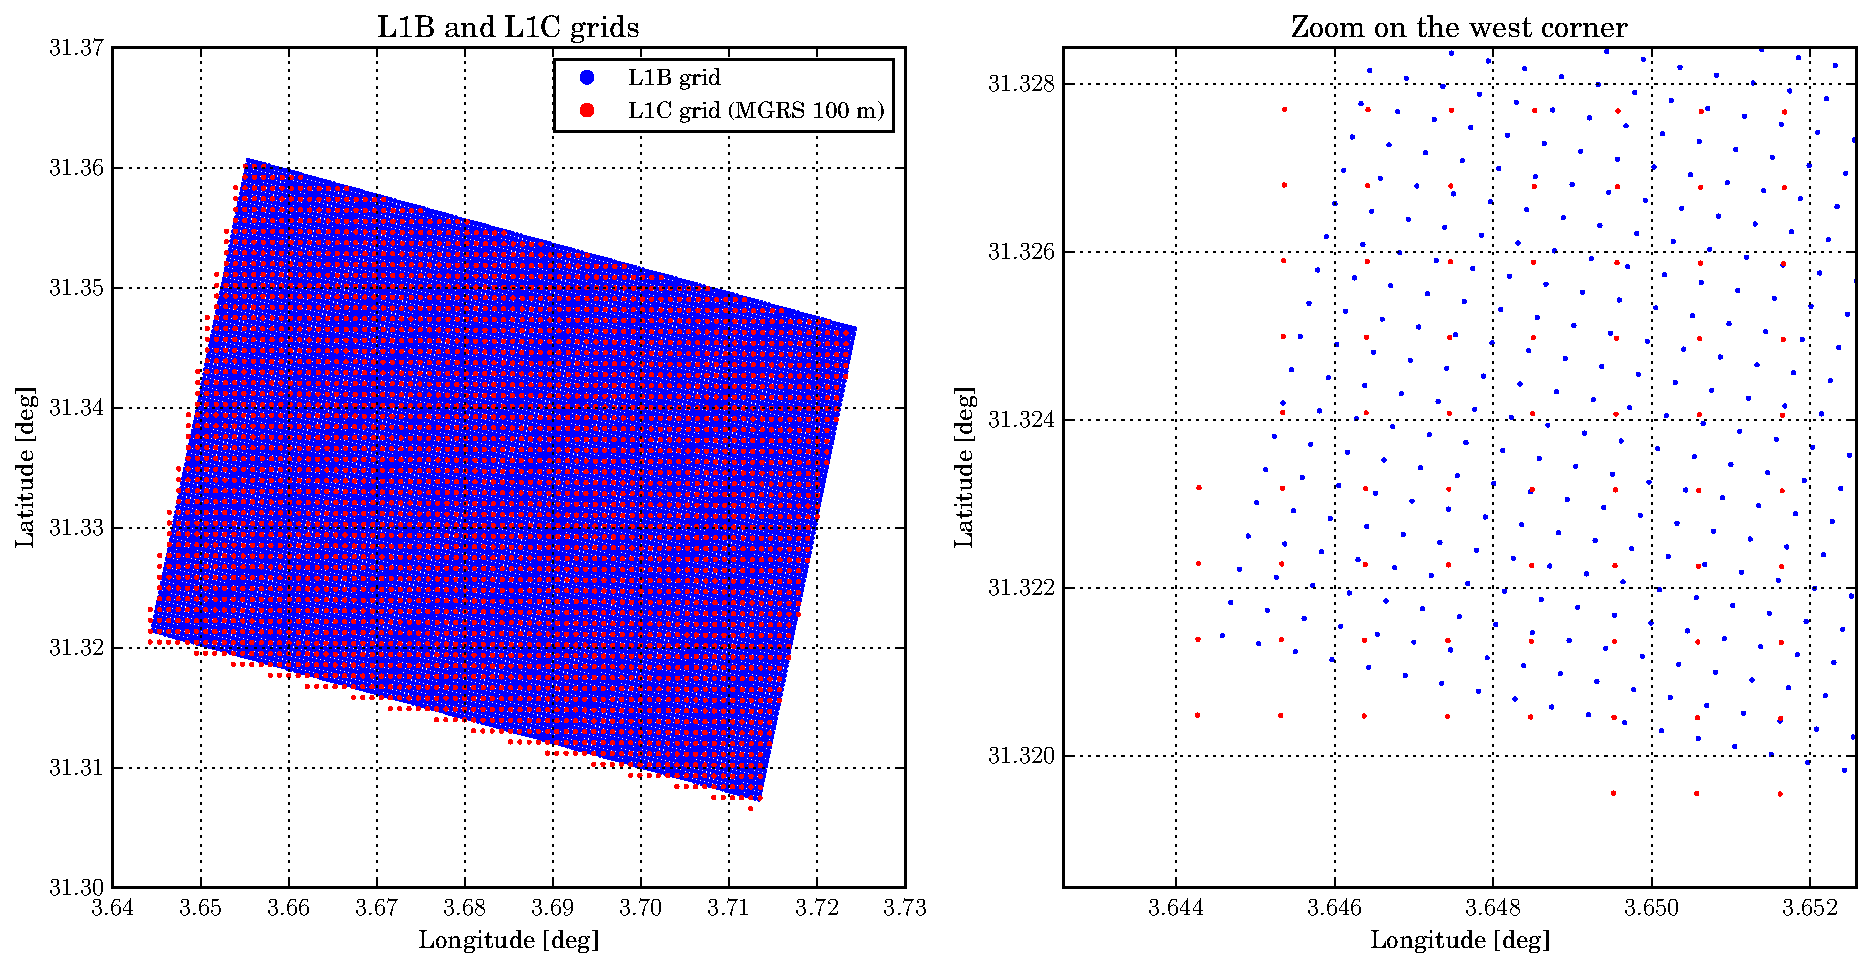
\includegraphics[width=\textwidth]{l1c_grids}
\caption{L1C. L1B and L1C grids. Full scene on the left and zoom on the west corner on the right.}
\label{fig:l1c_grids}
\end{figure}

\subsubsection{Ground sampling distance}
The GSD of the L1B is the distance on ground between consecutive pixels.
It is computed with the Haversine formula along the central line (ACT) and the central column (ALT).
Table~\ref{tab:l1c_gsd} and Figure~\ref{fig:l1c_gsd} show the result.

\begin{table}[H]
\centering
\caption{L1B ground sampling distance.}
\label{tab:l1c_gsd}
\begin{tabular}{lccc}
\toprule
Direction & Mean [m] & Min. [m] & Max. [m] \\
\midrule
ACT & 45.16 & 45.16 & 45.16 \\
ALT & 45.29 & 45.28 & 45.29 \\
\bottomrule
\end{tabular}

\end{table}

\begin{figure}[H]
\centering
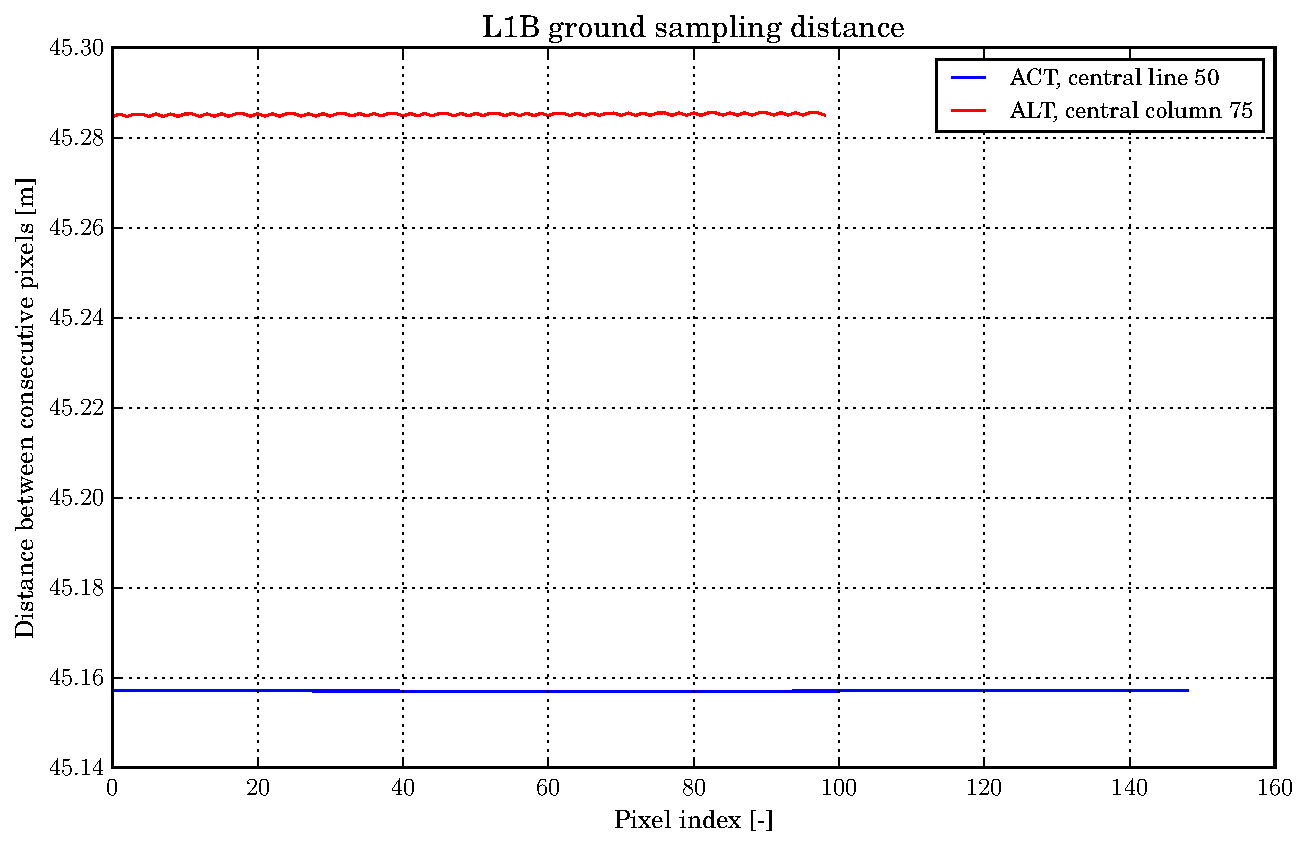
\includegraphics[width=0.75\textwidth]{l1c_gsd}
\caption{L1C. L1B ground sampling distance ACT and ALT.}
\label{fig:l1c_gsd}
\end{figure}

The GSD is about 45~m in both directions and it is almost constant over the scene.
Each L1B pixel covers about $45 \times 45 \approx 2045$~m$^2$. Each L1C tile covers $100 \times 100 = 10^4$~m$^2$.
The ratio is 4.9. Then $15000 / 4.9 \approx 3070$ tiles cover the scene. The rest of the 3129 tiles are on the borders, where tiles are only partly covered.

\subsubsection{L1C radiances}
Figures~\ref{fig:l1c_toa_0} to~\ref{fig:l1c_toa_3} compare the L1B and L1C radiances on the map.
The L1C keeps the gradient of the scene.
On the west border some L1C values differ from their neighbours. The south-west corner of these tiles is outside the L1B footprint, so the spline extrapolates. In VNIR-2 two points have a negative radiance for this reason.
A margin around the image or a check of the footprint would avoid it.

\begin{figure}[H]
\centering
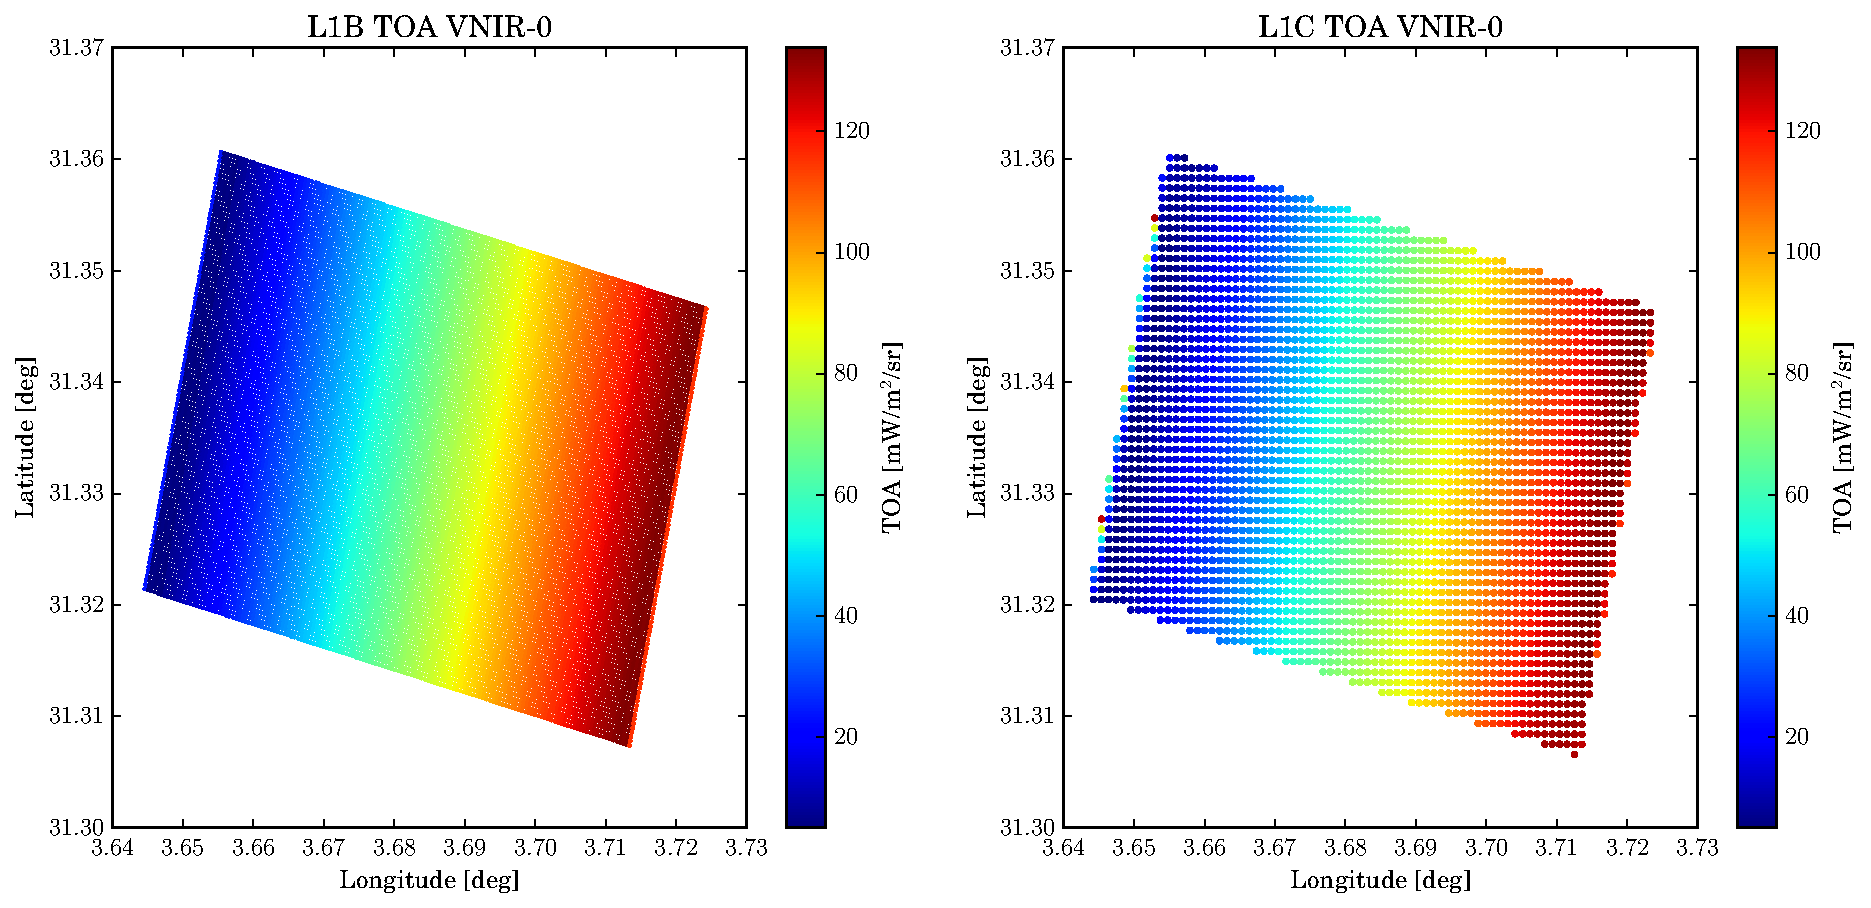
\includegraphics[width=\textwidth]{l1c_toa_map_VNIR-0}
\caption{L1C. L1B and L1C TOA, VNIR-0.}
\label{fig:l1c_toa_0}
\end{figure}

\begin{figure}[H]
\centering
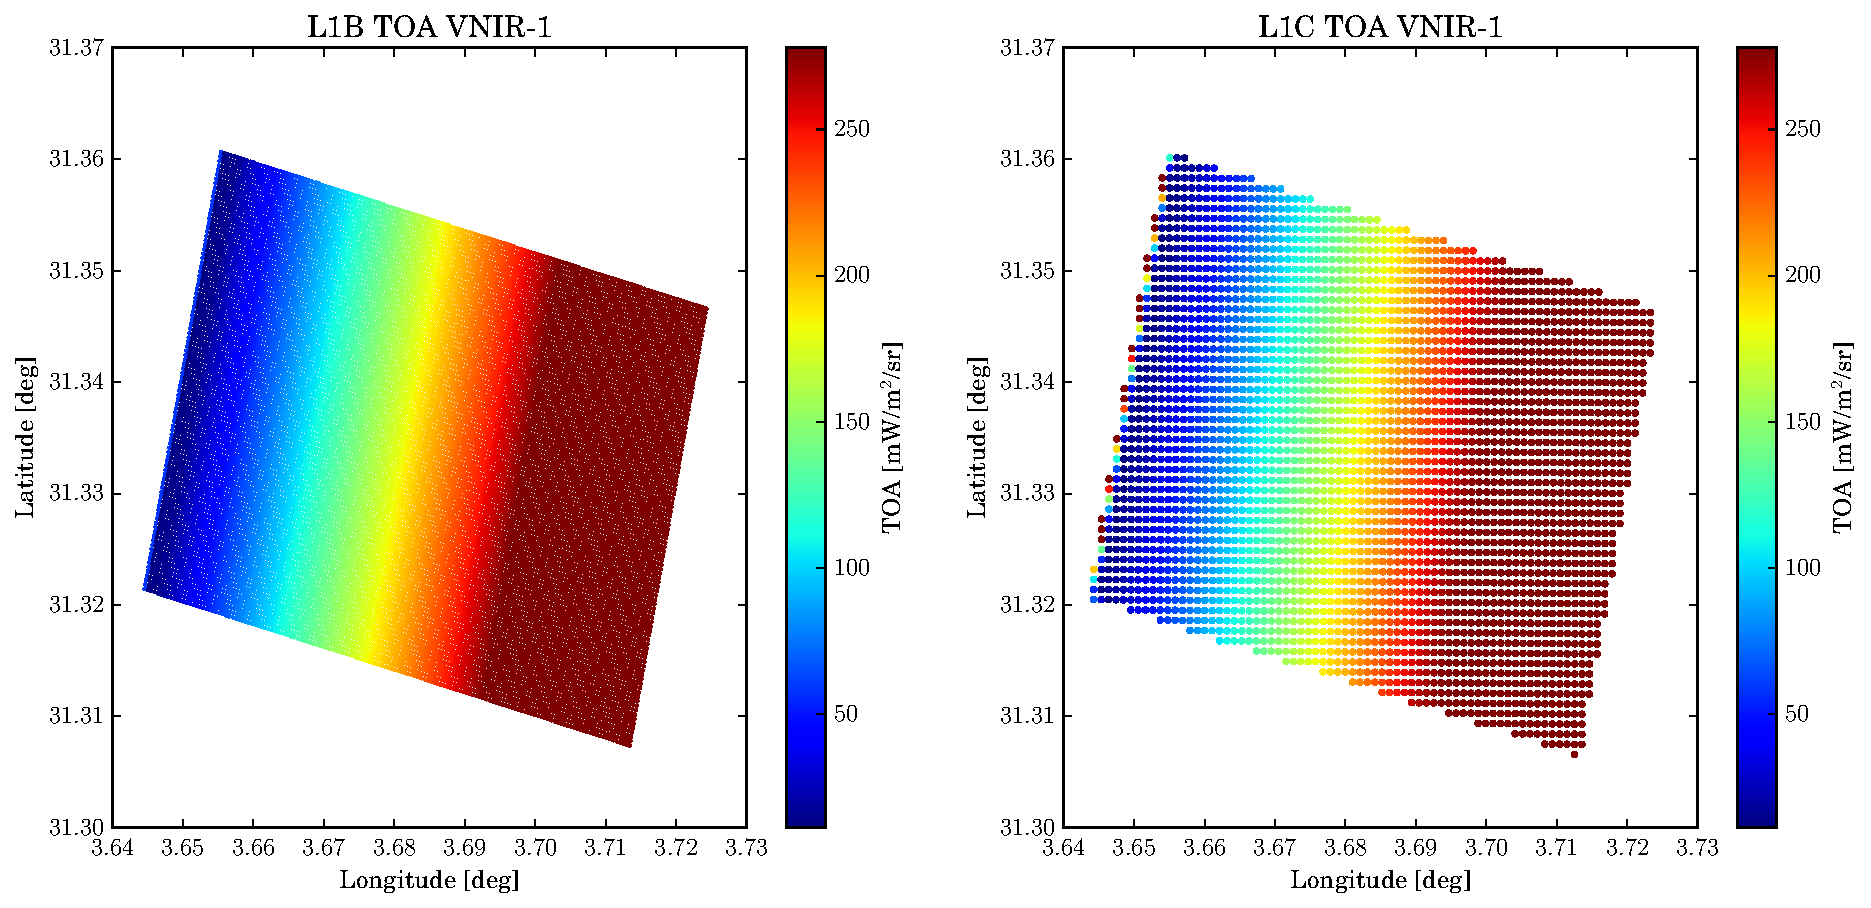
\includegraphics[width=\textwidth]{l1c_toa_map_VNIR-1}
\caption{L1C. L1B and L1C TOA, VNIR-1.}
\label{fig:l1c_toa_1}
\end{figure}

\begin{figure}[H]
\centering
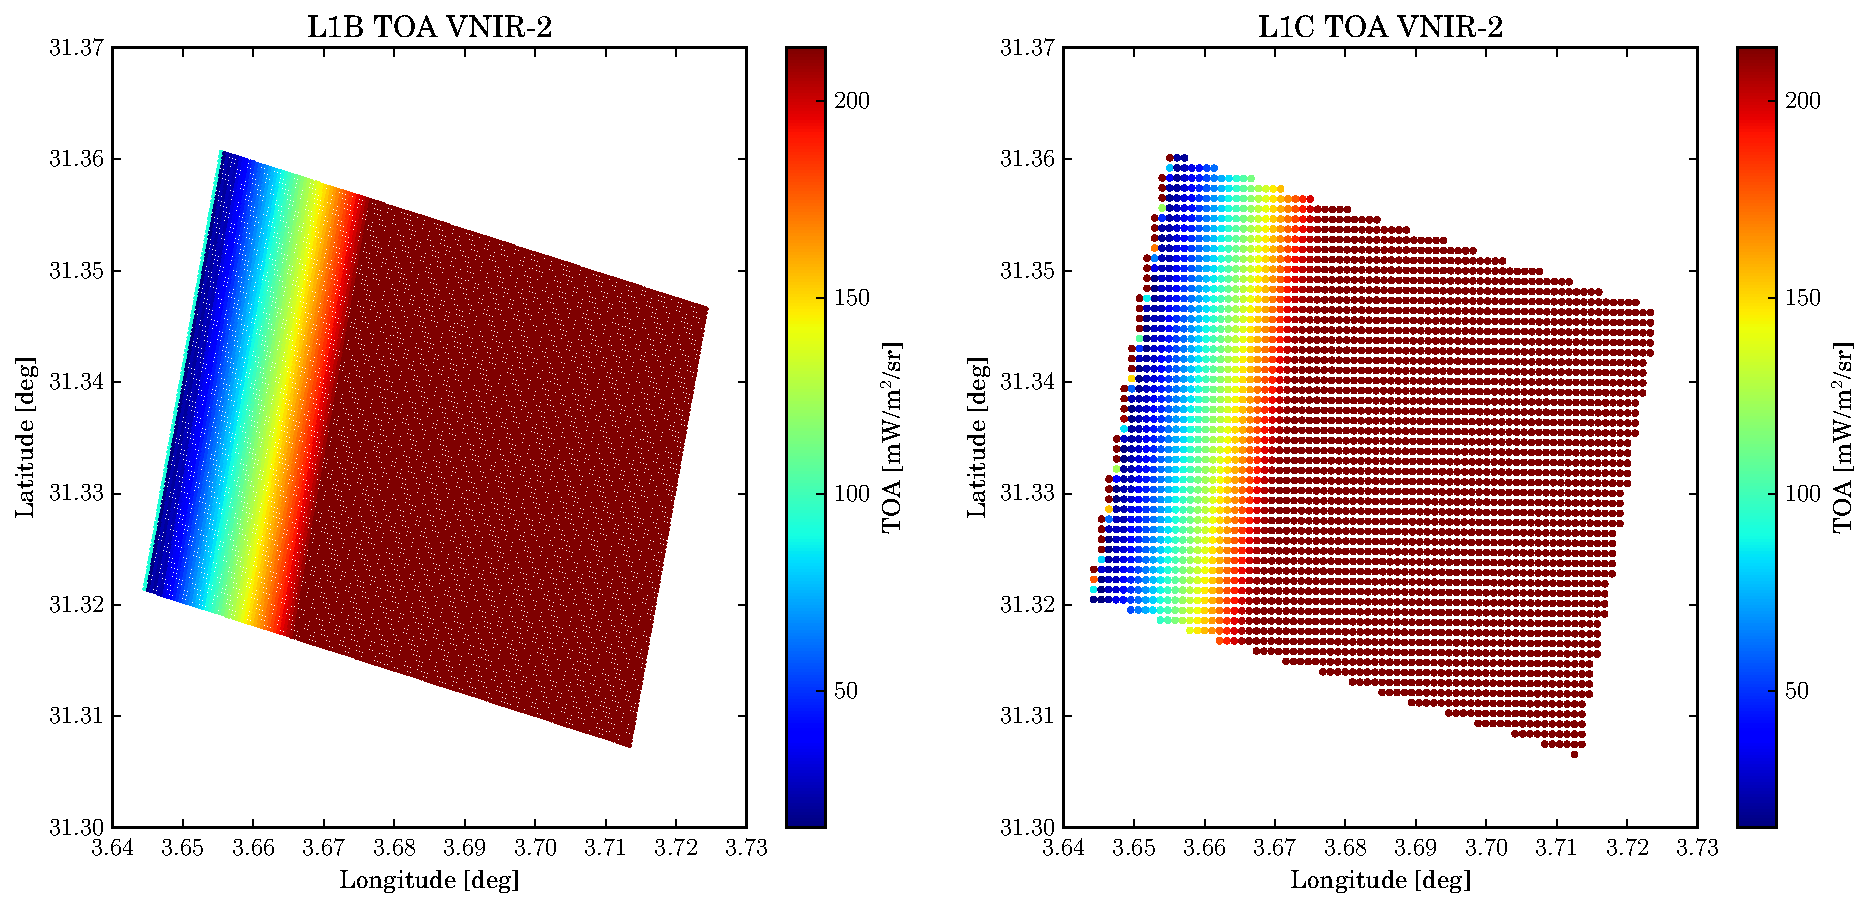
\includegraphics[width=\textwidth]{l1c_toa_map_VNIR-2}
\caption{L1C. L1B and L1C TOA, VNIR-2.}
\label{fig:l1c_toa_2}
\end{figure}

\begin{figure}[H]
\centering
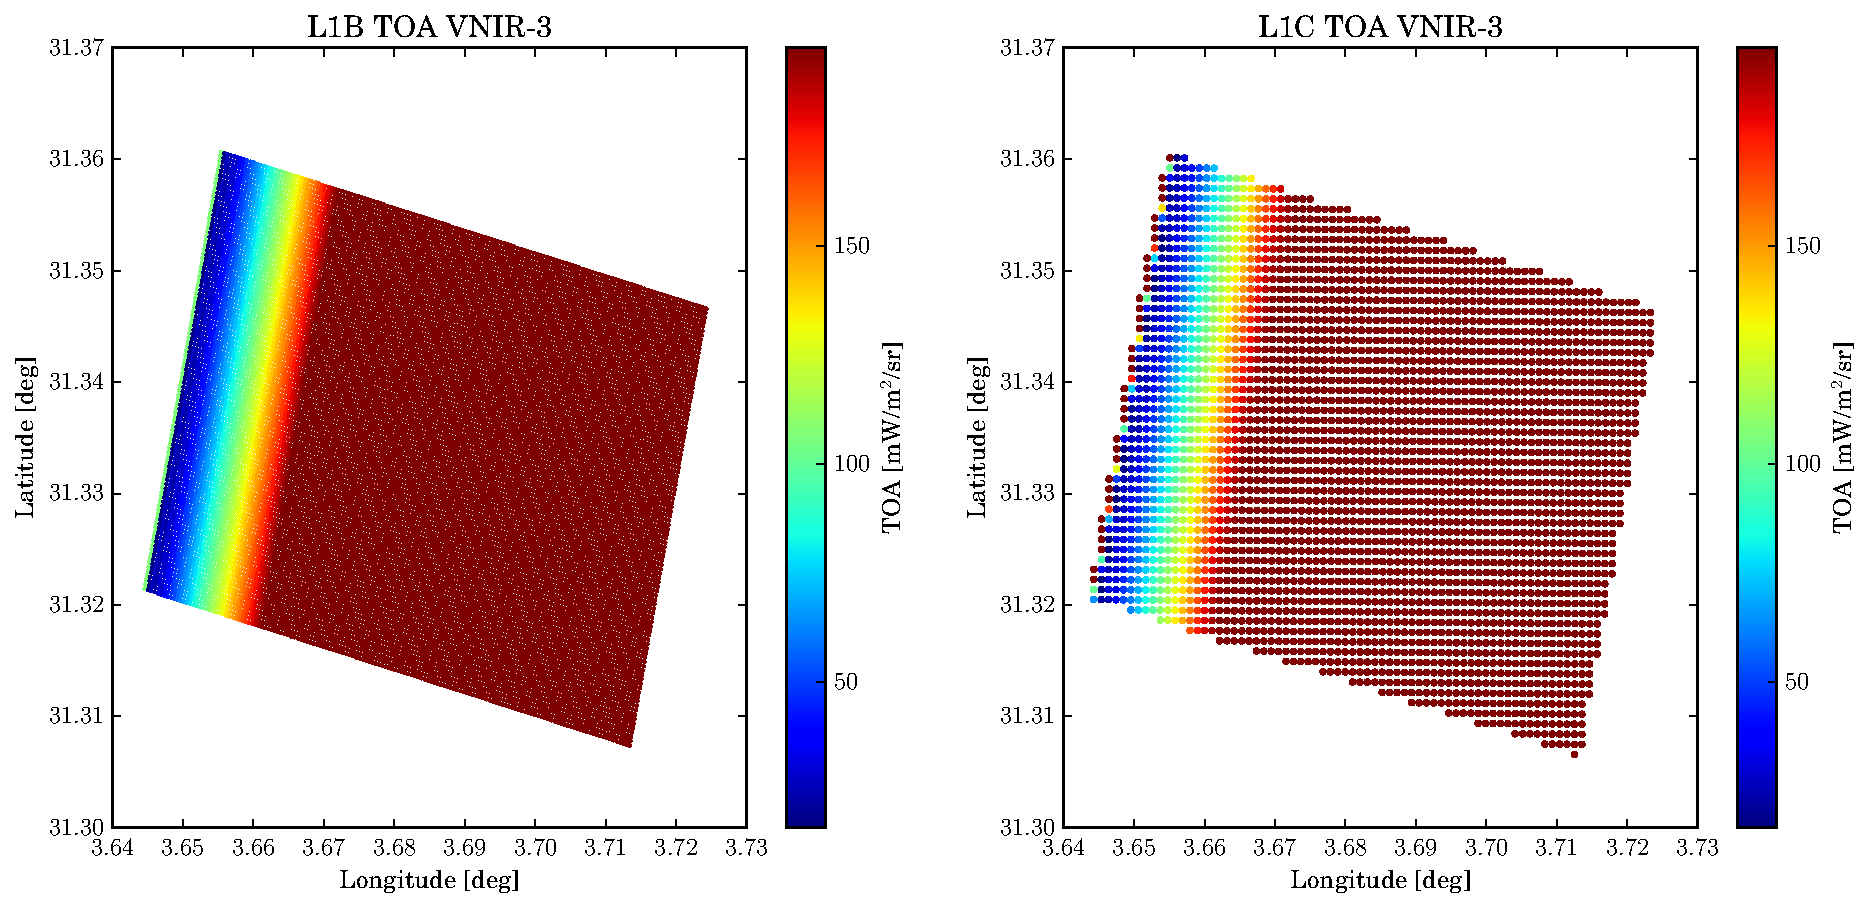
\includegraphics[width=\textwidth]{l1c_toa_map_VNIR-3}
\caption{L1C. L1B and L1C TOA, VNIR-3.}
\label{fig:l1c_toa_3}
\end{figure}

\subsection{Theoretical question. Processing levels and the need for the L1C}
The data of an EO mission are processed in levels.
\begin{itemize}
\item Level 0. Raw instrument packets in time order, as received on ground.
\item Level 1A. The packets are decoded into images in DN, with the time and the auxiliary data attached.
\item Level 1B. The DN are converted into radiances with the calibration. The image keeps the geometry of the sensor and each pixel has its geolocation.
\item Level 1C. The L1B radiances are resampled onto a fixed cartographic grid.
\item Level 2. Geophysical variables retrieved from the L1, such as reflectance, vegetation indices or fluorescence.
\end{itemize}

The L1B grid is different for each acquisition. It depends on the orbit, the attitude and the terrain.
Two L1B products of the same area cannot be compared pixel by pixel.
The L1C solves this. All the products are projected onto the same grid, so they can be stacked in time, combined with other sensors and used to build maps.
The L1B remains the most accurate radiance because it is not interpolated.

The grid used is the Military Grid Reference System (MGRS).
It is based on the UTM projection, which divides the Earth into 60 zones of $6^\circ$ in longitude. Each zone is a transverse Mercator projection with coordinates in metres.
MGRS divides each UTM zone into latitude bands of $8^\circ$ and squares of 100~km with two letters. Inside each square the easting and northing give the position. The number of digits fixes the precision.
In the code \texttt{31REQ660644} is zone 31, band R, square EQ, easting 660 and northing 644 in units of 100~m.

The L1C has fewer points than the L1B because the MGRS tile of 100~m is larger than the GSD of 45~m.
Several L1B pixels fall in the same tile and the tile is counted once.
The ideal grid size would be the SSD of the sensor. The configuration uses 100~m, as the ATBD recommends \cite{atbd}.

\subsection{Conclusion}
The L1C outputs match the reference after matching the points by coordinates.
The L1B GSD is 45.2~m ACT and 45.3~m ALT.
\textbf{EODP-TS-L1C: PASS.}

\section{EODP-TS-E2E. End-to-end test}
\label{sec:e2e}

\subsection{Objective}
The test runs the full chain on a real scene. The modules run in a row and each one reads the outputs of the previous one.
\begin{center}
SGM scene $\rightarrow$ ISM $\rightarrow$ L1B $\rightarrow$ L1C
\end{center}
The scene is a FLEX acquisition over the Pyrenees.
The test checks that the chain runs without errors and that the L1B recovers the input radiance.

\subsection{Inputs and configuration}
The ISM reads the scene in \texttt{EODP-TS-E2E/sgm\_out}. It has 951 lines, 525 columns and 650 wavelengths.
The L1C reads the geolocation in \texttt{EODP-TS-E2E/gm\_out} and the L1B output.
The configuration is the one of \texttt{EODP-TS-E2E/config}. Table~\ref{tab:e2e_config} shows the parameters that change with respect to the unitary tests.
The radiometric errors are disabled, so the L1B does not need the equalization.

\begin{table}[H]
\centering
\caption{E2E configuration. Parameters that differ from the unitary tests.}
\label{tab:e2e_config}
\begin{tabular}{lrr}
\toprule
Parameter & Unitary tests & E2E \\
\midrule
Pixel size $w$ & 30~\textmu m & 42~\textmu m \\
Integration time $t_{int}$ & 6.72~ms & 42.8~ms \\
Pupil diameter $D$ & 0.150~m & 0.07565~m \\
Focal length $f$ & 0.5262~m & 0.2345~m \\
PRNU, dark signal, bad and dead pixels & applied & not applied \\
L1B equalization & yes & no \\
L1B gain VNIR-0 [mW/m$^2$/sr/DN] & 0.0921 & 0.00576 \\
L1B gain VNIR-1 [mW/m$^2$/sr/DN] & 0.0679 & 0.00425 \\
L1B gain VNIR-2 [mW/m$^2$/sr/DN] & 0.0522 & 0.00326 \\
L1B gain VNIR-3 [mW/m$^2$/sr/DN] & 0.0478 & 0.00299 \\
\bottomrule
\end{tabular}
\end{table}

\subsection{Execution}
The script \texttt{harness/EODP-TS-E2E/test\_e2e.py} sets \texttt{EODP\_CONFIG\_DIR} to the E2E configuration and runs the three modules.
The ISM took 195~s, the L1B 11~s and the L1C 61~s. The three modules finished without errors.
As agreed in class, the report shows the L1B results only.

\subsection{Results}

\subsubsection{Altitude}
Figure~\ref{fig:e2e_altitude} shows the variable \texttt{altitude} of \texttt{gm\_out/geolocation.nc} on the map.
The geometry is the same for the four bands, so there is a single plot.
The altitude goes from 131~m to 2972~m. The Pyrenees cross the scene from west to east at about $42.6^\circ$N.

\begin{figure}[H]
\centering
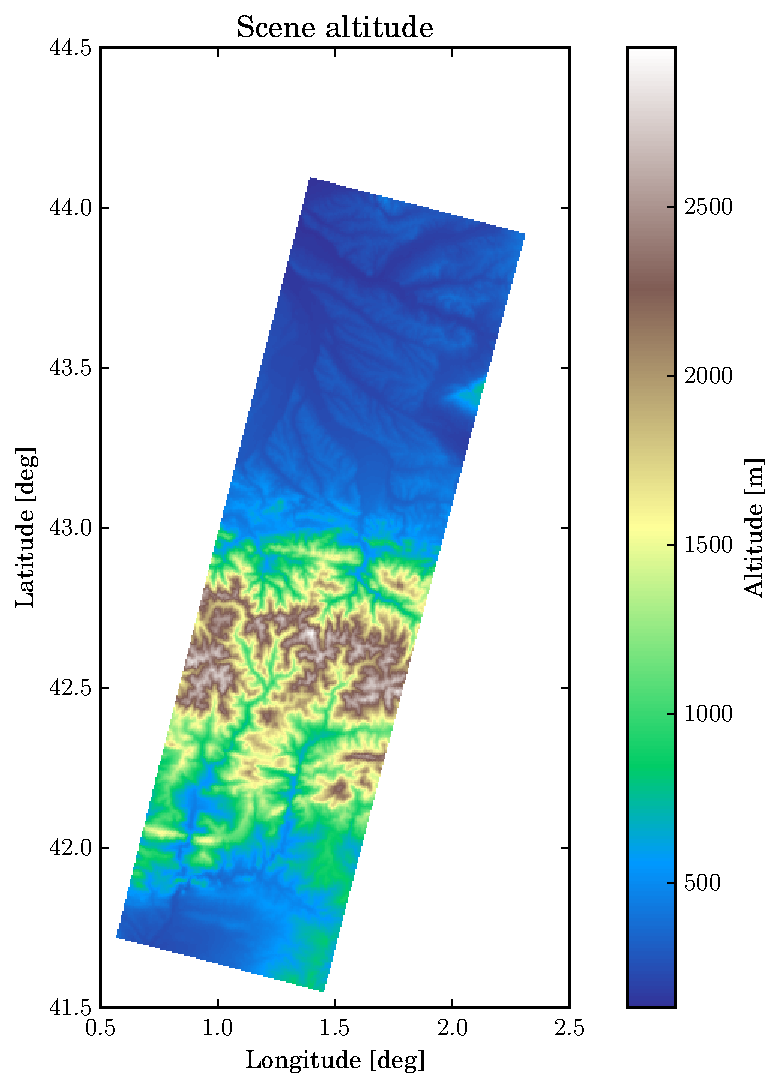
\includegraphics[width=0.7\textwidth]{e2e_altitude}
\caption{E2E. Altitude of the scene.}
\label{fig:e2e_altitude}
\end{figure}

\subsubsection{L1B radiances}
Figures~\ref{fig:e2e_0} to~\ref{fig:e2e_3} show the L1B TOA of each band on the map, with its histogram.
The histograms use bins of 0.1~mW/m$^2$/sr.
The same structures appear in the four bands. The lowest radiances are in the mountains, on the slopes in shadow.
VNIR-0 and VNIR-1 have the highest radiances, up to 13.7~mW/m$^2$/sr. VNIR-2 and VNIR-3 reach 7.1 and 8.5~mW/m$^2$/sr.
The histograms are consistent with the maps. Most pixels are bright and a long tail on the left comes from the shadowed mountain areas.

\begin{figure}[H]
\centering
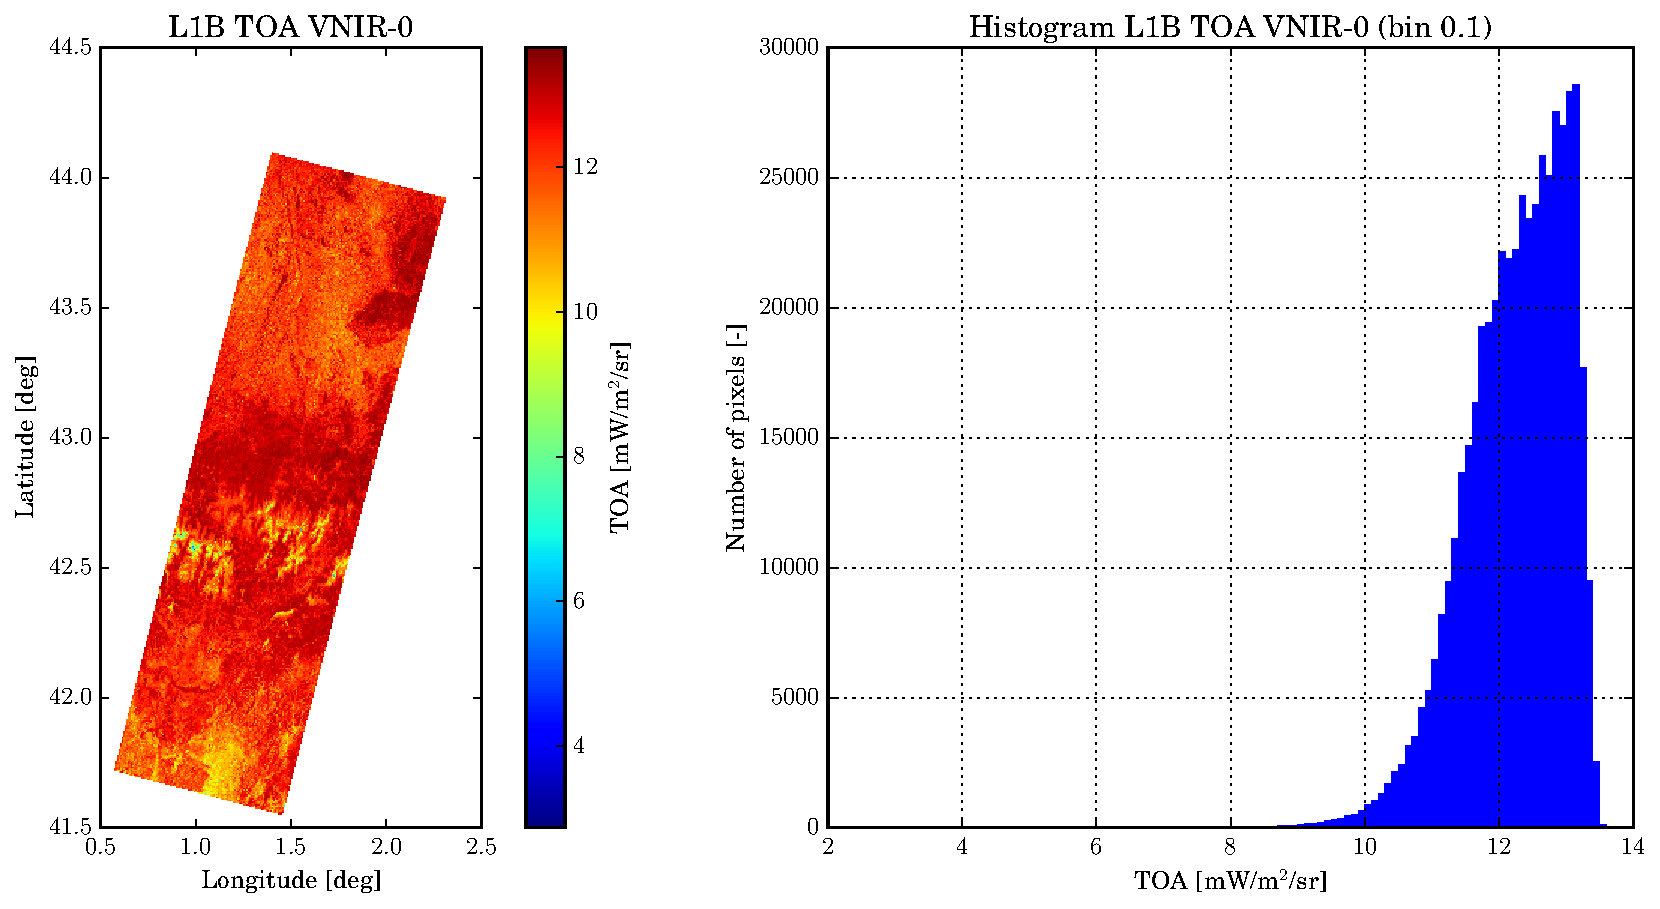
\includegraphics[width=\textwidth]{e2e_l1b_VNIR-0}
\caption{E2E. L1B TOA and histogram, VNIR-0.}
\label{fig:e2e_0}
\end{figure}

\begin{figure}[H]
\centering
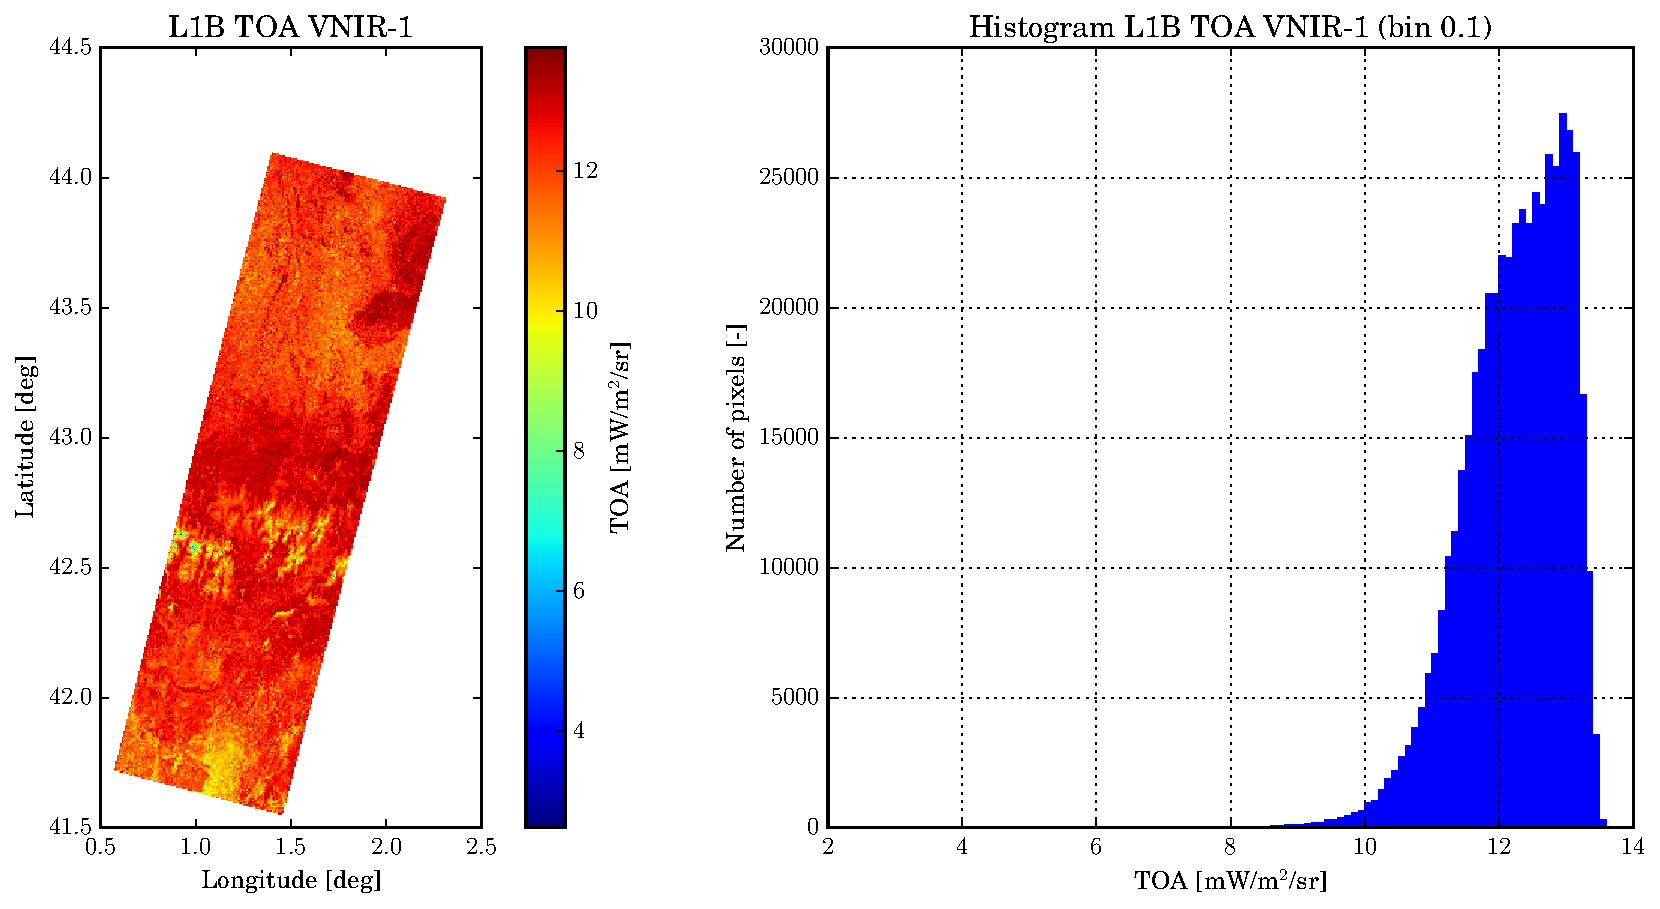
\includegraphics[width=\textwidth]{e2e_l1b_VNIR-1}
\caption{E2E. L1B TOA and histogram, VNIR-1.}
\label{fig:e2e_1}
\end{figure}

\begin{figure}[H]
\centering
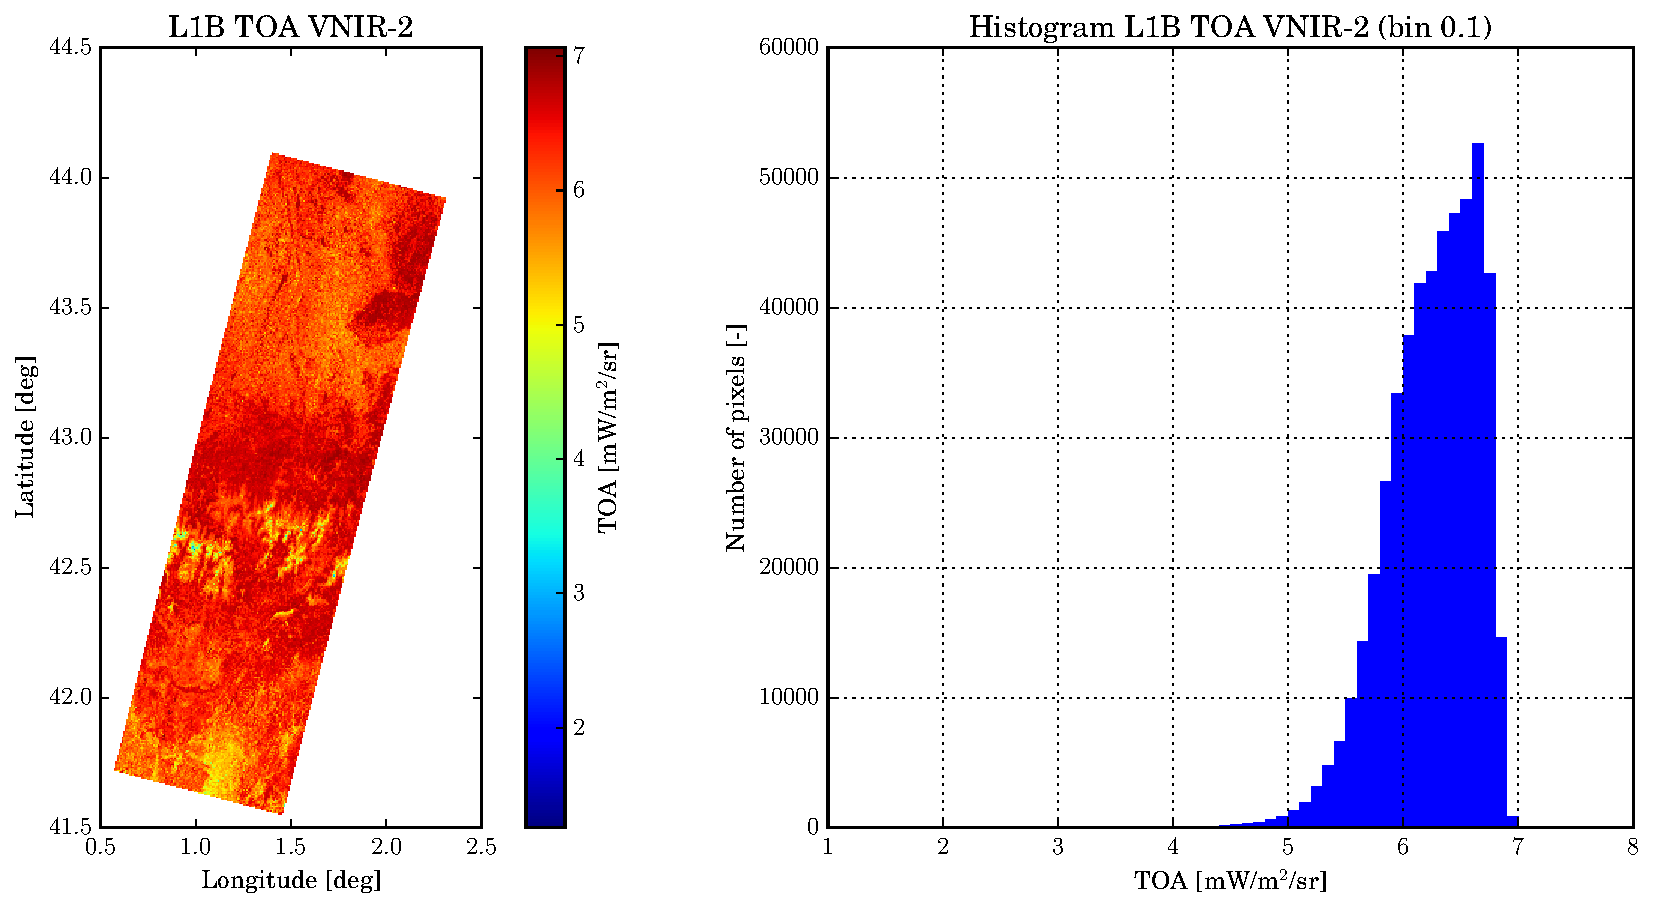
\includegraphics[width=\textwidth]{e2e_l1b_VNIR-2}
\caption{E2E. L1B TOA and histogram, VNIR-2.}
\label{fig:e2e_2}
\end{figure}

\begin{figure}[H]
\centering
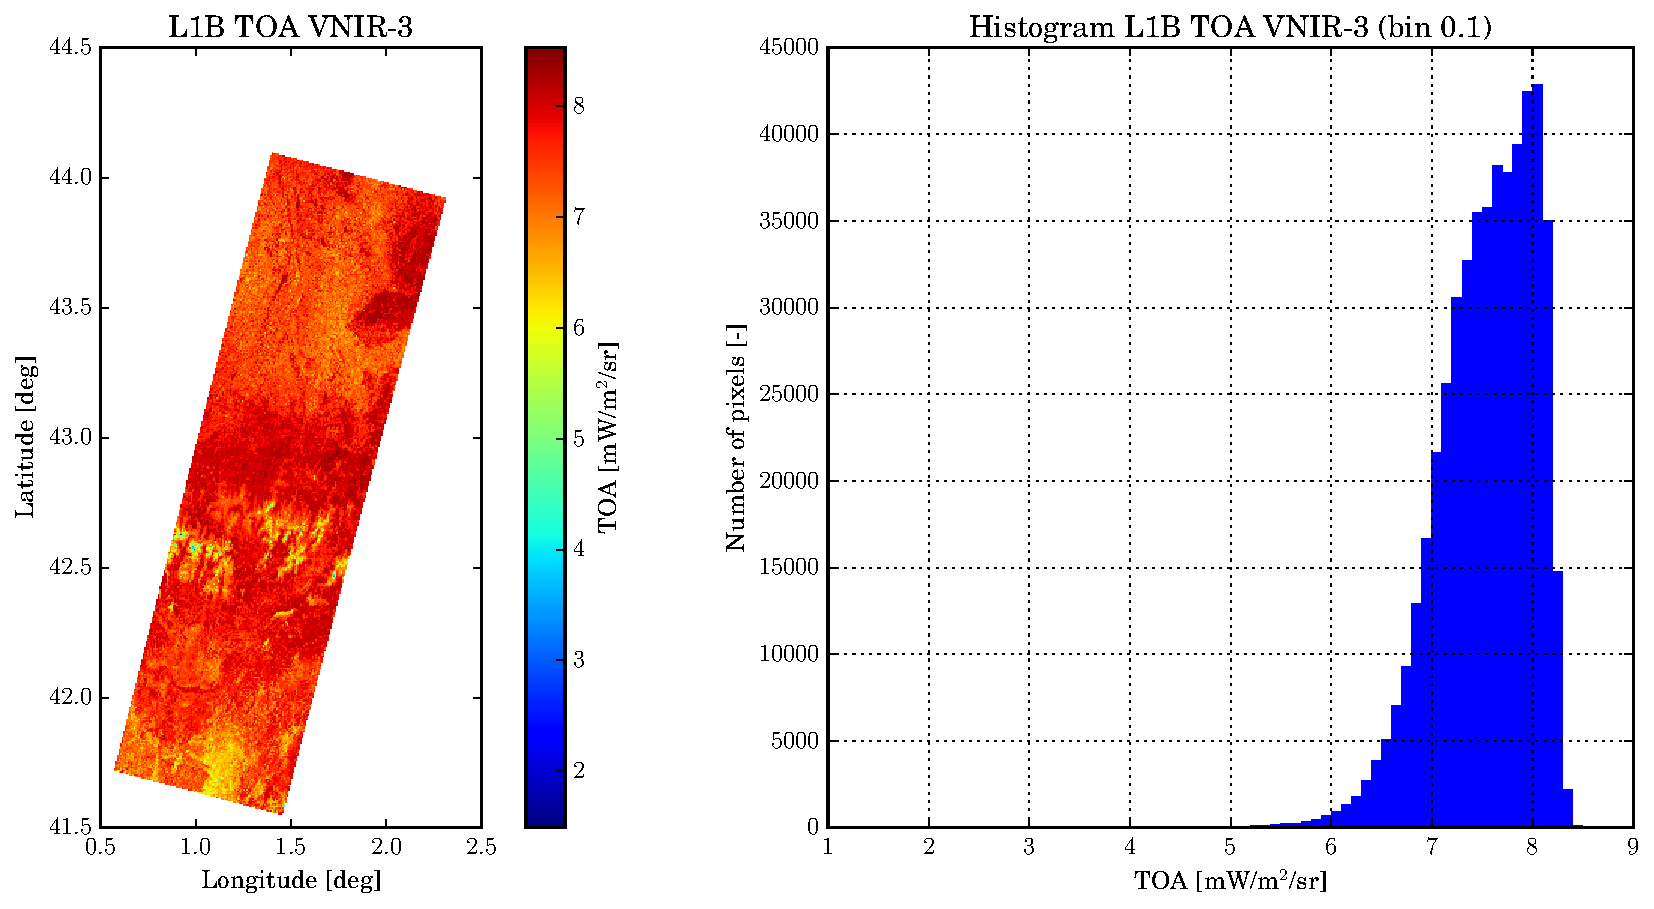
\includegraphics[width=\textwidth]{e2e_l1b_VNIR-3}
\caption{E2E. L1B TOA and histogram, VNIR-3.}
\label{fig:e2e_3}
\end{figure}

\subsubsection{Radiometric consistency}
Without radiometric errors, the L1B should recover the radiance that enters the instrument.
Table~\ref{tab:e2e_radiometry} compares the mean of \texttt{ism\_toa\_isrf} with the mean of \texttt{l1b\_toa}.
The difference is about $-0.02\,\%$ in all the bands. It comes from the MTF and the quantisation.
No pixel is saturated.

\begin{table}[H]
\centering
\caption{E2E. Mean radiance before the instrument and after the L1B [mW/m$^2$/sr].}
\label{tab:e2e_radiometry}
\begin{tabular}{lcccc}
\toprule
Band & Mean ISRF TOA & Mean L1B TOA & Difference [\%] & Saturated [\%] \\
\midrule
VNIR-0 & 12.2554 & 12.2529 & -0.021 & 0.00 \\
VNIR-1 & 12.2348 & 12.2326 & -0.018 & 0.00 \\
VNIR-2 & 6.2529 & 6.2520 & -0.016 & 0.00 \\
VNIR-3 & 7.5464 & 7.5453 & -0.015 & 0.00 \\
\bottomrule
\end{tabular}

\end{table}

As an additional check, the ISM and L1B outputs were compared with the outputs provided with the E2E data.
Table~\ref{tab:e2e_crossval} shows that they are identical within $1.2\times10^{-5}\,\%$.

\begin{longtable}{lccccc}
\caption{E2E. Comparison with the ISM and L1B outputs provided with the E2E data. Maximum relative difference [\%] per band.}\label{tab:e2e_crossval}\\
\toprule
File & VNIR-0 & VNIR-1 & VNIR-2 & VNIR-3 & Result \\
\midrule
\endfirsthead
\toprule
File & VNIR-0 & VNIR-1 & VNIR-2 & VNIR-3 & Result \\
\midrule
\endhead
\texttt{ism\_toa\_isrf\_} & $0$ & $0$ & $0$ & $0$ & Pass \\
\texttt{ism\_toa\_optical\_} & $0$ & $0$ & $0$ & $0$ & Pass \\
\texttt{ism\_toa\_e\_} & $0$ & $0$ & $0$ & $0$ & Pass \\
\texttt{ism\_toa\_detection\_} & $0$ & $0$ & $0$ & $0$ & Pass \\
\texttt{ism\_toa\_} & $0$ & $0$ & $0$ & $0$ & Pass \\
\texttt{l1b\_toa\_} & $1.18\times10^{-5}$ & $1.19\times10^{-5}$ & $1.19\times10^{-5}$ & $1.19\times10^{-5}$ & Pass \\
\bottomrule
\end{longtable}


\subsection{Conclusion}
The chain ISM, L1B and L1C runs without errors on the real scene.
The L1B recovers the mean input radiance within 0.02~\%.
\textbf{EODP-TS-E2E: PASS.}

\section{Conclusions}
\label{sec:conclusions}

Table~\ref{tab:summary} summarises the results.

\begin{table}[H]
\centering
\caption{Summary of the tests.}
\label{tab:summary}
\begin{tabular}{llc}
\toprule
Test & Evidence & Result \\
\midrule
EODP-TS-ISM & 28 TOA files and 28 MTF files equal to the reference & Pass \\
EODP-TS-L1B & 8 files equal to the reference & Pass \\
EODP-TS-L1C & 4 files equal to the reference after matching the points & Pass \\
EODP-TS-E2E & Chain without errors. Mean radiance recovered within 0.02~\% & Pass \\
\bottomrule
\end{tabular}
\end{table}

The main findings are the following.
\begin{itemize}
\item All the outputs of the unitary tests match the reference with a relative difference below $10^{-3}\,\%$. Most of them are identical.
\item The detector MTF defines the system MTF in VNIR-1, VNIR-2 and VNIR-3. The wavefront error aberrations define it in VNIR-0. The system MTF at Nyquist is between 0.36 and 0.45.
\item The two largest unit conversion factors are the irradiance to photons and the volts to DN conversions. The MTF, the detection effects and the saturation explain why the analytic conversion differs from the saved outputs.
\item In the unitary test scene VNIR-1, VNIR-2 and VNIR-3 saturate. The L1B cannot recover the radiance above the saturation level.
\item The equalization removes the PRNU and DSNU stripes. The L1B then follows the input radiance.
\item The L1B GSD is about 45~m. The L1C grid of 100~m has fewer points than the L1B. Near the borders the L1C spline extrapolates.
\item The end-to-end chain works on a real scene. The L1B recovers the input radiance.
\end{itemize}

Two improvements are suggested.
A margin around the image would remove the MTF edge effect of the ISM.
A check of the L1B footprint in the L1C would avoid the extrapolated values on the borders.


\bibliographystyle{plain}
\bibliography{references}

\end{document}
